% Scilab ( http://www.scilab.org/ ) - This file is part of Scilab
% Copyright (C) 2008-2010 - Digiteo - Michael Baudin
%
% This file must be used under the terms of the CeCILL.
% This source file is licensed as described in the file COPYING, which
% you should have received as part of this distribution.  The terms
% are also available at
% http://www.cecill.info/licences/Licence_CeCILL_V2-en.txt

\documentclass[12pt]{article}

% Scilab ( http://www.scilab.org/ ) - This file is part of Scilab
% Copyright (C) 2008-2010 - Digiteo - Michael Baudin
%
% This file must be used under the terms of the CeCILL.
% This source file is licensed as described in the file COPYING, which
% you should have received as part of this distribution.  The terms
% are also available at
% http://www.cecill.info/licences/Licence_CeCILL_V2-en.txt

%% Good fonts for PDF
\usepackage[cyr]{aeguill}

\usepackage{amsmath,amsopn}

%% Package for page headers
\usepackage{fancyhdr}

%%% package for conditionals in TeX
\usepackage{ifthen}                 

%% Index
\usepackage{makeidx}
\makeindex

%% Package to include graphics
%% Comment for DVI
\usepackage[pdftex]{graphicx}

%% Figures formats: jpeg or pdf
%% Comment for DVI
\DeclareGraphicsExtensions{.jpg,.pdf}

%% Package to create Hyperdocuments
%% Comment for DVI
% urls
\usepackage[pdftex,bookmarks=true,bookmarksnumbered=true,breaklinks=true,
hypertexnames=false,colorlinks=true,linkcolor=blue,citecolor=blue,urlcolor=blue]{hyperref}

%%%%%%%%%%%%%%%%%%%%%%%%%%%%%%%%%%%%%%%%%%%%%%%%%%%%%%%%%% PDFLATEX %%%
%%%
\usepackage[pdftex]{thumbpdf}      %%% thumbnails for pdflatex


%% Package to control printed area size
\usepackage{anysize}
%% ...by defining margins {left}{right}{top}{bottom}
\marginsize{22mm}{14mm}{12mm}{25mm}

%% Package used to include a bibliography
\usepackage{natbib}

%% R for real numbers
\usepackage{amssymb}

%% User defined commands

%% Figure reference
\newcommand{\figref}[1]{figure~\ref{#1}}

%% Equation reference
\newcommand{\Ref}[1]{(\ref{#1})}

%% Emphasize a word or a group of words
\newcommand{\empha}[1]{\textit{\textbf{#1}}}

%% Derivation operators
\newcommand{\D}{\partial}
\newcommand{\Dt}{\partial_t}
\newcommand{\Dx}{\partial_x}
\newcommand{\Dy}{\partial_y}

% Scilab macros
%\newcommand{\scimacro}[1]{\textit{#1}}
%\newcommand{\scifunction}[1]{\texttt{#1}}
\newcommand{\scifun}[1]{\texttt{#1}}
\newcommand{\scivar}[1]{\texttt{#1}}
\newcommand{\scifile}[1]{\texttt{#1}}
\newcommand{\sourcefile}[1]{\texttt{#1}}
\newcommand{\cvar}[1]{\texttt{#1}}
\newcommand{\terminalcommand}[1]{\texttt{#1}}
\newcommand{\cfunction}[1]{\texttt{#1}}
\newcommand{\scimenu}[1]{\textit{#1}}
\newcommand{\scisinglequote}{{"\hspace{0.1cm}\scivar{'}\hspace{0.1cm}"}}
\newcommand{\scidoublequote}{{"\hspace{0.1cm}\scivar{"}\hspace{0.1cm}"}}
\newcommand{\sciewisesinglequote}{{"\hspace{0.1cm}\scivar{.'}\hspace{0.1cm}"}}


% Maths shortcuts 
% Double barred letters
\newcommand{\RR}{\mathbb{R}}
\newcommand{\CC}{\mathbb{C}}
\newcommand{\NN}{\mathbb{N}}
\newcommand{\ZZ}{\mathbb{Z}}

\newcommand{\ba}{\mathbf{a}}
\newcommand{\bb}{\mathbf{b}}
\newcommand{\bd}{\mathbf{d}}
\newcommand{\be}{\mathbf{e}}
\newcommand{\boldf}{\mathbf{f}}
\newcommand{\bp}{\mathbf{p}}
\newcommand{\bg}{\mathbf{g}}
\newcommand{\bq}{\mathbf{q}}
\newcommand{\bu}{\mathbf{u}}
\newcommand{\bv}{\mathbf{v}}
\newcommand{\bw}{\mathbf{w}}
\newcommand{\bx}{\mathbf{x}}
\newcommand{\by}{\mathbf{y}}
\newcommand{\bz}{\mathbf{z}}
\newcommand{\bH}{\mathbf{H}}
\newcommand{\bzero}{\mathbf{0}}

% Machine epsilon
\newcommand{\epsmach}{\epsilon_M}

% Scalar product
\newcommand{\scapro}[2]{<#1,#2>}


% Binomial coefficient
\newcommand{\choosefun}[2]{
\left(
\begin{array}{@{}c@{}}
#1\\
#2
\end{array}
\right)
}


% To highlight source code
\usepackage{listings}

% To allow one bibliograph by chapter
%\usepackage[sectionbib]{chapterbib}
\usepackage{url}
\usepackage{amsthm}


% Some environments
\newtheorem{theorem}{Theorem}[section]
\newtheorem{lemma}[theorem]{Lemma}
\newtheorem{proposition}[theorem]{Proposition}
\newtheorem{corollary}[theorem]{Corollary}
\newtheorem{axiom}[theorem]{Axiom}
\newtheorem{definition}[theorem]{Definition}
\newtheorem{remark}[theorem]{Remark}


\newtheoremstyle{examplestyle}
  {0.2cm}{0cm}%                                 margin top and bottom
  {\rmfamily}%                                  text layout
  {0cm}%                                        indention of header
  {\bfseries}%                                  header font
  {}%                                           and text after header
  {0cm}%                                        space after header
  {\thmname{#1}\thmnumber{ #2} }%  header
\theoremstyle{examplestyle}
\newtheorem{example}{Example}[section]


% Algorithms
\usepackage{algorithmic}
\usepackage{algorithm2e}



\lstdefinelanguage{scilabscript}%
  {morekeywords={abcd,abinv,abort,abs,acoshm,acosh,acosm,acos,addcolor,%
      addf,addinter,addmenu,add_edge,add_node,adj2sp,adj_lists,aff2ab,%
      amell,analpf,analyze,ans,apropos,arc_graph,arc_number,argn,arhnk,%
      arl2,arma2p,armac,armax1,armax,arma,arsimul,artest,articul,ascii,%
      asinhm,asinh,asinm,asin,atanhm,atanh,atanm,atan,augment,auread,%
      auwrite,balanc,balreal,bandwr,basename,bdiag,besseli,besselj,%
      besselk,bessely,best_match,bezout,bifish,bilin,binomial,black,%
      bloc2exp,bloc2ss,bode,bool2s,boolean,boucle,break,bstap,buttmag,%
      bvode,cainv,calerf,calfrq,call,canon,casc,case,ccontrg,cdfbet,%
      cdfbin,cdfchi,cdfchn,cdffnc,cdff,cdfgam,cdfnbn,cdfnor,cdfpoi,%
      cdft,ceil,center,cepstrum,chaintest,chain_struct,champ1,champ,%
      chart,chdir,cheb1mag,cheb2mag,check_graph,check_io,chepol,chfact,%
      chol,chsolve,circuit,classmarkov,clean,clearfun,clearglobal,%
      clear,close,cls2dls,cmb_lin,cmndred,cmoment,code2str,coeff,coffg,%
      coff,colcompr,colcomp,colinout,colormap,colregul,companion,comp,%
      cond,conj,connex,contour2di,contour2d,contourf,contour,%
      contract_edge,contrss,contr,cont_frm,cont_mat,convex_hull,convol,%
      convstr,con_nodes,copfac,copy,correl,corr,coshm,cosh,cosm,cos,%
      cotg,cothm,coth,covar,csim,cspect,ctr_gram,cumprod,cumsum,%
      curblock,cycle_basis,czt,c_link,dasrt,dassl,datafit,date,dbphi,%
      dcf,ddp,debug,dec2hex,deff,definedfields,degree,delbpt,%
      delete_arcs,delete_nodes,delete,delip,delmenu,demos,denom,%
      derivative,derivat,des2ss,des2tf,determ,detr,det,dft,dhinf,%
      dhnorm,diag,diary,diff,diophant,dirname,dispbpt,dispfiles,disp,%
      dlgamma,double,dragrect,drawaxis,drawlater,drawnow,draw,driver,%
      dscr,dsearch,dsimul,dtsi,dt_ility,duplicate,edge_number,%
      edit_curv,edit_graph_menus,edit_graph,edit,eigenmarkov,ell1mag,%
      elseif,else,emptystr,endfunction,end,eqfir,eqiir,equil1,equil,%
      ereduc,erfcx,erfc,erf,errbar,errcatch,errclear,error,eval3dp,%
      eval3d,eval,evans,evstr,excel2sci,execstr,exec,exists,exit,expm,%
      exp,external,eye,fac3d,factors,faurre,fchamp,fcontour2d,fcontour,%
      fec,feedback,feval,ffilt,fftshift,fft,fgrayplot,figure,fileinfo,%
      file,filter,findm,findobj,findx0BD,find_freq,find_path,find,%
      findABCD,findAC,findBD,findBDK,findR,fit_dat,fix,floor,flts,foo,%
      formatman,format,fort,for,fourplan,fplot2d,fplot3d1,fplot3d,%
      fprintf,fprintfMat,frep2tf,freq,freson,frexp,frfit,frmag,fscanf,%
      fscanfMat,fsfirlin,fsolve,fspecg,fstabst,fstair,ftest,ftuneq,%
      fullrfk,fullrf,full,fun2string,funcprot,functions,function,%
      funptr,fusee,gainplot,gamitg,gammaln,gamma,gcare,gcd,gcf,%
      genfac3d,genlib,genmarkov,gen_net,geom3d,geomean,getblocklabel,%
      getcolor,getcurblock,getcwd,getdate,getd,getenv,getfield,getfont,%
      getf,getio,getlinestyle,getmark,getpid,getscicosvars,getsymbol,%
      getvalue,getversion,get_function_path,get,gfare,gfrancis,girth,%
      givens,glever,glist,global,glue,gpeche,graduate,grand,%
      graphics_entities,graph_2_mat,graph_center,graph_complement,%
      graph_diameter,graph_power,graph_simp,graph_sum,graph_union,%
      graph-list,graycolormap,grayplot,graypolarplot,grep,group,%
      gr_menu,gschur,gsort,gspec,gstacksize,gtild,g_margin,h2norm,halt,%
      hamilton,hankelsv,hank,harmean,havewindow,help,hermit,hess,%
      hex2dec,hilb,hinf,hist3d,histplot,horner,host,hotcolormap,%
      householder,hrmt,htrianr,hypermat,h_cl,h_inf_st,h_inf,h_norm,%
      iconvert,icon_edit,ieee,if,iirgroup,iirlp,iir,ilib_build,%
      ilib_compile,ilib_for_link,ilib_gen_gateway,ilib_gen_loader,%
      ilib_gen_Make,imag,impl,imrep2ss,imult,im_inv,inistate,input,%
      int16,int2d,int32,int3d,int8,intc,intdec,integrate,interpln,%
      interp,intersci,intersect,intg,intl,intppty,intsplin,inttrap,%
      inttype,int,invr,invsyslin,inv_coeff,inv,iqr,isdef,isdir,isequal,%
      iserror,isglobal,isinf,isnan,isoview,isreal,is_connex,jmat,%
      justify,kalm,karmarkar,kernel,keyboard,knapsack,kpure,krac2,%
      kroneck,kron,lasterror,lattn,lattp,lcf,lcmdiag,lcm,ldivf,ldiv,%
      leastsq,legends,length,leqr,levin,lev,lex_sort,lft,lgfft,library,%
      lib,lin2mu,lincos,lindquist,lines,line_graph,linfn,linf,link,%
      linmeq,linpro,linsolve,linspace,lin,listfiles,list,lmisolver,%
      lmitool,loadmatfile,loadplots,loadwave,load_graph,load,locate,%
      log10,log1p,log2,logm,logspace,log,lotest,lqe,lqg2stan,lqg_ltr,%
      lqg,lqr,lsq,lsslist,lstcat,lstsize,ltitr,ludel,lufact,luget,%
      lusolve,lu,lyap,macglov,macr2lst,macrovar,macro,mad,make_graph,%
      make_index,manedit,man,mapsound,markp2ss,matfile2sci,matrix,%
      mat_2_graph,maxi,max_cap_path,max_clique,max_flow,max,mclearerr,%
      mclose,meanf,mean,median,meof,mese,mesh2d,mfft,mfile2sci,mgeti,%
      mgetl,mgetstr,mget,milk_drop,mine,mini,minreal,minss,%
      min_lcost_cflow,min_lcost_flow1,min_lcost_flow2,min_qcost_flow,%
      min_weight_tree,min,mlist,mode,modulo,moment,mopen,move,%
      mps2linpro,mputl,mputstr,mput,mrfit,msd,mseek,mtell,mtlb_load,%
      mtlb_mode,mtlb_save,mtlb_sparse,mu2lin,mulf,mvvacov,m_circle,%
      names,nand2mean,nanmax,nanmeanf,nanmean,nanmedian,nanmin,%
      nanstdev,nansum,narsimul,ndims,nearfloat,nehari,neighbors,%
      netclose,netwindows,netwindow,newest,newfun,nextpow2,nf3d,nfreq,%
      nlev,nnz,nodes_2_path,nodes_degrees,node_number,noisegen,norm,%
      null,numdiff,numer,nyquist,obscont1,obscont,observer,obsvss,%
      obsv_mat,obs_gram,odedc,odedi,odeoptions,ode_discrete,ode_root,%
      ode,oldload,oldsave,ones,optim,orth,param3d1,param3d,%
      paramfplot2d,parrot,part,pathconvert,path_2_nodes,pause,pbig,%
      pdiv,pen2ea,pencan,penlaur,perctl,perfect_match,pertrans,pfss,%
      phasemag,phc,pinv,pipe_network,playsnd,plot2d1,plot2d2,plot2d3,%
      plot2d4,plot2d,plot3d1,plot3d2,plot3d3,plot3d,plotframe,%
      plotprofile,plot_graph,plot,plzr,pmodulo,pol2des,pol2str,pol2tex,%
      polarplot,polar,polfact,poly,portr3d,portrait,power,ppol,prbs_a,%
      predecessors,predef,printf,printing,print,prod,profile,projsl,%
      projspec,proj,psmall,pspect,pvm_addhosts,pvm_barrier,pvm_bcast,%
      pvm_bufinfo,pvm_config,pvm_delhosts,pvm_error,pvm_exit,%
      pvm_f772sci,pvm_getinst,pvm_gettid,pvm_get_timer,pvm_gsize,%
      pvm_halt,pvm_joingroup,pvm_kill,pvm_lvgroup,pvm_mytid,pvm_parent,%
      pvm_probe,pvm_recv,pvm_reduce,pvm_sci2f77,pvm_send,pvm_set_timer,%
      pvm_spawn_independent,pvm_spawn,pvm_start,pvm_tasks,%
      pvm_tidtohost,pvm,pwd,p_margin,qassign,qr,quapro,quart,quaskro,%
      quit,randpencil,rand,range,rankqr,rank,rat,rcond,rdivf,read4b,%
      readb,readc_,readmps,read,real,recur,reglin,regress,remezb,remez,%
      repfreq,replot,residu,resume,return,riccati,riccsl,ricc,ric_desc,%
      rlist,roots,rotate,round,routh_t,rowcompr,rowcomp,rowinout,%
      rowregul,rowshuff,rpem,rref,rtitr,rubberbox,salesman,savewave,%
      save_graph,save,scaling,scanf,schur,sci2exp,sci2for,sci2map,%
      sciargs,scicosim,scicos,scifunc_block,sd2sci,secto3d,select,%
      semidef,sensi,setbpt,seteventhandler,setfield,setmenu,%
      setscicosvars,set,sfact,sgrid,shortest_path,showprofile,%
      show_arcs,show_graph,show_nodes,sident,signm,sign,simp_mode,simp,%
      sincd,sinc,sinc,sinhm,sinh,sinm,sin,size,sm2des,sm2ss,smooth,%
      solve,sorder,sort,sound,sp2adj,spaninter,spanplus,spantwo,sparse,%
      spchol,spcompack,specfact,spec,speye,spget,splin,split_edge,%
      spones,sprand,sprintf,spzeros,sqroot,sqrtm,sqrt,squarewave,%
      square,srfaur,srkf,ss2des,ss2ss,ss2tf,sscanf,sskf,ssprint,ssrand,%
      stabil,stacksize,standard_define,standard_draw,standard_input,%
      standard_origin,standard_output,startup,stdevf,stdev,steadycos,%
      str2code,strange,strcat,strindex,strings,string,stripblanks,%
      strong_connex,strong_con_nodes,strsubst,st_deviation,st_ility,%
      subf,subgraph,subplot,successors,sum,supernode,sva,svd,svplot,%
      sylm,sylv,sysconv,sysdiag,sysfact,syslin,syssize,systems,system,%
      systmat,tabul,tangent,tanhm,tanh,tanm,tan,tdinit,testmatrix,%
      texprint,tf2des,tf2ss,then,thrownan,timer,time_id,titlepage,%
      tk_getdir,tk_getfile,tlist,toeplitz,tokenpos,tokens,trace,%
      translatepaths,trans_closure,trans,trfmod,trianfml,tril,trimmean,%
      trisolve,triu,trzeros,typename,typeof,type,uicontrol,uimenu,%
      uint16,uint32,uint8,ui_observer,ulink,unglue,union,unique,unix_g,%
      unix_s,unix_w,unix_x,unix,unobs,unsetmenu,user,varargin,%
      varargout,variancef,variance,varn,warning,wavread,wavwrite,%
      wcenter,wfir,what,whereami,whereis,where,while,whos,who_user,who,%
      wiener,wigner,window,winsid,with_gtk,with_pvm,with_texmacs,%
      with_tk,writb,write4b,write,xarcs,xarc,xarrows,xaxis,xbasc,%
      xbasimp,xbasr,xchange,xclear,xclea,xclick,xclip,xdel,xend,xfarcs,%
      xfarc,xfpolys,xfpoly,xfrect,xgetech,xgetfile,xgetmouse,xget,%
      xgraduate,xgrid,xinfo,xinit,xlfont,xload,xname,xnumb,xpause,%
      xpolys,xpoly,xrects,xrect,xrpoly,xs2fig,xs2gif,xs2ppm,xs2ps,%
      xsave,xsegs,select,xsetech,xsetm,xset,xstringb,xstringl,xstring,%
      xtape,xtitle,x_choices,x_choose,x_dialog,x_matrix,x_mdialog,%
      x_message_modeless,x_message,yulewalk,zeropen,zeros,zgrid,zpbutt,%
      zpch1,zpch2,zpell,mfprintf,mfscanf,mprintf,mscanf,msprintf,%
      msscanf,mucomp,%
      ABSBLK_f,AFFICH_f,ANDLOG_f,ANIMXY_f,BIGSOM_f,CLINDUMMY_f,CLKIN_f,%
      CLKINV_f,CLKOUT_f,CLKOUTV_f,CLKSOM_f,CLKSOMV_f,CLKSPLIT_f,%
      CLOCK_f,CLR_f,CLSS_f,CONST_f,COSBLK_f,CURV_f,DELAY_f,DELAYV_f,%
      DEMUX_f,DLR_f,DLRADAPT_f,DLSS_f,EVENTSCOPE_f,EVTDLY_f,EVTGEN_f,%
      EXPBLK_f,G_make,GAIN_f,GAINBLK_f,GENERAL_f,GENERIC_f,GENSIN_f,%
      GENSQR_f,HALT_f,IFTHEL_f,IN_f,INTEGRAL_f,INTRP2BLK_f,INTRPLBLK_f,%
      INVBLK_f,LOGBLK_f,LOOKUP_f,Matplot1,Matplot,MAX_f,MCLOCK_f,%
      MFCLCK_f,MIN_f,MUX_f,NDcost,NEGTOPOS_f,OUT_f,POSTONEG_f,POWBLK_f,%
      PROD_f,QUANT_f,RAND_f,READC_f,REGISTER_f,RELAY_f,RFILE_f,%
      ScilabEval,Sfgrayplot,Sgrayplot,SAMPLEHOLD_f,SAT_f,SAWTOOTH_f,%
      SCOPE_f,SCOPXY_f,SELECT_f,SINBLK_f,SOM_f,SPLIT_f,STOP_f,SUPER_f,%
      TANBLK_f,TCLSS_f,TEXT_f,TIME_f,TK_EvalFile,TK_EvalStr,TK_GetVar,%
      TK_SetVar,TRASH_f,WFILE_f,WRITEC_f,ZCROSS_f,%
      \%asn,\%helps,\%k,\%sn},%
   alsoletter=\%,% chmod
   sensitive,%
   morecomment=[l]//,%
   morestring=[b]",%
   morestring=[m]'%
   numbers=none,%
   basicstyle=\footnotesize\ttfamily,%
   keywordstyle=\bfseries,%
   commentstyle=\bfseries,%
   showspaces=false,%
   showstringspaces=false,%
   stringstyle=\bfseries, 
   %framexleftmargin=13mm,
   %backgroundcolor=\color{grey}, %% TOO MUCH INK !
   xleftmargin=12mm,
   %, frameround={tttt}
   %captionpos=b,
   %frame = single % or shadowbox or lines %% Frame the source code
  }[keywords,comments,strings]%

\lstdefinelanguage{matlabscript}%
  {morekeywords={gt,lt,gt,lt,amp,abs,acos,acosh,acot,acoth,acsc,acsch,%
      all,angle,ans,any,asec,asech,asin,asinh,atan,atan2,atanh,auread,%
      auwrite,axes,axis,balance,bar,bessel,besselk,bessely,beta,%
      betainc,betaln,blanks,bone,break,brighten,capture,cart2pol,%
      cart2sph,caxis,cd,cdf2rdf,cedit,ceil,chol,cla,clabel,clc,clear,%
      clf,clock,close,colmmd,Colon,colorbar,colormap,ColorSpec,colperm,%
      comet,comet3,compan,compass,computer,cond,condest,conj,contour,%
      contour3,contourc,contrast,conv,conv2,cool,copper,corrcoef,cos,%
      cosh,cot,coth,cov,cplxpair,cputime,cross,csc,csch,csvread,%
      csvwrite,cumprod,cumsum,cylinder,date,dbclear,dbcont,dbdown,%
      dbquit,dbstack,dbstatus,dbstep,dbstop,dbtype,dbup,ddeadv,ddeexec,%
      ddeinit,ddepoke,ddereq,ddeterm,ddeunadv,deblank,dec2hex,deconv,%
      del2,delete,demo,det,diag,diary,diff,diffuse,dir,disp,dlmread,%
      dlmwrite,dmperm,dot,drawnow,echo,eig,ellipj,ellipke,else,elseif,%
      end,engClose,engEvalString,engGetFull,engGetMatrix,engOpen,%
      engOutputBuffer,engPutFull,engPutMatrix,engSetEvalCallback,%
      engSetEvalTimeout,engWinInit,eps,erf,erfc,erfcx,erfinv,error,%
      errorbar,etime,etree,eval,exist,exp,expint,expm,expo,eye,fclose,%
      feather,feof,ferror,feval,fft,fft2,fftshift,fgetl,fgets,figure,%
      fill,fill3,filter,filter2,find,findstr,finite,fix,flag,fliplr,%
      flipud,floor,flops,fmin,fmins,fopen,for,format,fplot,fprintf,%
      fread,frewind,fscanf,fseek,ftell,full,function,funm,fwrite,fzero,%
      gallery,gamma,gammainc,gammaln,gca,gcd,gcf,gco,get,getenv,%
      getframe,ginput,global,gplot,gradient,gray,graymon,grid,griddata,%
      gtext,hadamard,hankel,help,hess,hex2dec,hex2num,hidden,hilb,hist,%
      hold,home,hostid,hot,hsv,hsv2rgb,if,ifft,ifft2,imag,image,%
      imagesc,Inf,info,input,int2str,interp1,interp2,interpft,inv,%
      invhilb,isempty,isglobal,ishold,isieee,isinf,isletter,isnan,%
      isreal,isspace,issparse,isstr,jet,keyboard,kron,lasterr,lcm,%
      legend,legendre,length,lin2mu,line,linspace,load,log,log10,log2,%
      loglog,logm,logspace,lookfor,lower,ls,lscov,lu,magic,matClose,%
      matDeleteMatrix,matGetDir,matGetFp,matGetFull,matGetMatrix,%
      matGetNextMatrix,matGetString,matlabrc,matlabroot,matOpen,%
      matPutFull,matPutMatrix,matPutString,max,mean,median,menu,mesh,%
      meshc,meshgrid,meshz,mexAtExit,mexCallMATLAB,mexdebug,%
      mexErrMsgTxt,mexEvalString,mexFunction,mexGetFull,mexGetMatrix,%
      mexGetMatrixPtr,mexPrintf,mexPutFull,mexPutMatrix,mexSetTrapFlag,%
      min,more,movie,moviein,mu2lin,mxCalloc,mxCopyCharacterToPtr,%
      mxCopyComplex16ToPtr,mxCopyInteger4ToPtr,mxCopyPtrToCharacter,%
      mxCopyPtrToComplex16,mxCopyPtrToInteger4,mxCopyPtrToReal8,%
      mxCopyReal8ToPtr,mxCreateFull,mxCreateSparse,mxCreateString,%
      mxFree,mxFreeMatrix,mxGetIr,mxGetJc,mxGetM,mxGetN,mxGetName,%
      mxGetNzmax,mxGetPi,mxGetPr,mxGetScalar,mxGetString,mxIsComplex,%
      mxIsFull,mxIsNumeric,mxIsSparse,mxIsString,mxIsTypeDouble,%
      mxSetIr,mxSetJc,mxSetM,mxSetN,mxSetName,mxSetNzmax,mxSetPi,%
      mxSetPr,NaN,nargchk,nargin,nargout,newplot,nextpow2,nnls,nnz,%
      nonzeros,norm,normest,null,num2str,nzmax,ode23,ode45,orient,orth,%
      pack,pascal,patch,path,pause,pcolor,pi,pink,pinv,plot,plot3,%
      pol2cart,polar,poly,polyder,polyeig,polyfit,polyval,polyvalm,%
      pow2,print,printopt,prism,prod,pwd,qr,qrdelete,qrinsert,quad,%
      quad8,quit,quiver,qz,rand,randn,randperm,rank,rat,rats,rbbox,%
      rcond,real,realmax,realmin,refresh,rem,reset,reshape,residue,%
      return,rgb2hsv,rgbplot,rootobject,roots,rose,rosser,rot90,rotate,%
      round,rref,rrefmovie,rsf2csf,save,saxis,schur,sec,sech,semilogx,%
      semilogy,set,setstr,shading,sign,sin,sinh,size,slice,sort,sound,%
      spalloc,sparse,spaugment,spconvert,spdiags,specular,speye,spfun,%
      sph2cart,sphere,spinmap,spline,spones,spparms,sprandn,sprandsym,%
      sprank,sprintf,spy,sqrt,sqrtm,sscanf,stairs,startup,std,stem,%
      str2mat,str2num,strcmp,strings,strrep,strtok,subplot,subscribe,%
      subspace,sum,surf,surface,surfc,surfl,surfnorm,svd,symbfact,%
      symmmd,symrcm,tan,tanh,tempdir,tempname,terminal,text,tic,title,%
      toc,toeplitz,trace,trapz,tril,triu,type,uicontrol,uigetfile,%
      uimenu,uiputfile,unix,unwrap,upper,vander,ver,version,view,%
      viewmtx,waitforbuttonpress,waterfall,wavread,wavwrite,what,%
      whatsnew,which,while,white,whitebg,who,whos,wilkinson,wk1read,%
      wk1write,xlabel,xor,ylabel,zeros,zlabel,zoom},%
   sensitive,%
   morecomment=[l]\%,%
   basicstyle=\footnotesize\ttfamily,%
   morestring=[m]',%
   xleftmargin=12mm
  }[keywords,comments,strings]%

\lstdefinelanguage{datafile}%
  {morekeywords={},%
   alsoletter=\%,% chmod
   sensitive,%
   morecomment=[l]//,%
   morestring=[b]",%
   morestring=[m]'%
   numbers=none,%
   basicstyle=\footnotesize\ttfamily,%
   keywordstyle=\bfseries,%
   commentstyle=\bfseries,%
   showspaces=false,%
   stringstyle=\bfseries, 
   %framexleftmargin=13mm,
   %backgroundcolor=\color{grey}, %% TOO MUCH INK !
   xleftmargin=12mm,
   %, frameround={tttt}
   %captionpos=b,
   frame = single % or shadowbox or lines %% Frame the source code
  }[keywords,comments,strings]%

% Least common multiple
\DeclareMathOperator{\lcm}{lcm} 


% Extend margins
\usepackage[hmargin=3cm,vmargin=3cm]{geometry}




\begin{document}
\author{Micha\"el Baudin}
\date{January 2010}
\title{Introduction to discrete probabilities with Scilab}

\maketitle

\begin{abstract}
In this article, we present an introduction to discrete probabilities with Scilab.
Numerical experiments are based on Scilab.
The first section present discrete random variables and 
conditionnal probabilities. In the second section, we present combinations problems,  
tree diagrams and Bernouilli trials. In the third section, we present simulation
of random processes with Scilab. 
\end{abstract}

\tableofcontents

% Copyright (C) 2008-2010 - Consortium Scilab - Digiteo - Michael Baudin
%
% This file must be used under the terms of the 
% Creative Commons Attribution-ShareAlike 3.0 Unported License :
% http://creativecommons.org/licenses/by-sa/3.0/


%%%%%%%%%%%%%%%%%%%%%%%%%%%%%%%%%%%%%%%%%%%%%%%%%%%%%%%%%%%%%%%%%%%%%%%%%%%%%%%%%%%%%%%

\section{Discrete random variables}
\label{idp-section-discrandvar}

In this section, we present discrete random variables.
The first section presents general definition for sets, including
union, intersection.
Then we present the definition of the discrete distribution
function and the probability of an event.
In the third section, we give properties of probabilities, 
such as, for example, the probability of the union of two disjoints 
events.
The fourth section is devoted to the very common 
discrete uniform distribution function.
Then we present the definition of conditional probability.

%%%%%%%%%%%%%%%%%%%%%%%%%%%%%%%%%%%%%%%%%%%%%%%%%%%%%%%%%%%%%%%%%%%%%%%%%%%%%%%%%%%%%%%
\subsection{Sets}
\label{introstats-setsrandomvars}
A \emph{set} is a collection of elements. In this document, we 
consider sets of elements in a fixed non empty set $\Omega$, to be 
called a \emph{space}.

Assume that $A$ is a set of elements. If $x$ 
is a point in that set, we note $x\in A$. 
If there is no point in $A$, we write $A=\emptyset$.
If the number of elements in $A$ is finite, let us denote by $\#(A)$ the number of 
elements in the set $A$. If the number of elements in $A$ is infinite, the 
cardinality cannot be computed (for example $A=\NN$).

The set $A^c$ is the set of all points in $\Omega$ which are not in $A$:
\begin{eqnarray}
A^c = \left\{x\in \Omega\; / \; x\notin A\right\}.
\end{eqnarray}
\index{complementary}
The set $A^c$ is called the \emph{complementary} set of $A$.

\index{subset}
The set $B$ is a \emph{subset} of $A$ if 
any point in $B$ is also in $A$ and we can write $A\subset B$.
The two sets $A$ and $B$ are equal if $A\subset B$ and $B\subset A$.
The difference set $A-B$ is the set of all points of $A$ which are 
not in $B$:
\begin{eqnarray}
A-B = \left\{x\in A \; / \; x\notin B\right\}.
\end{eqnarray}
\index{intersection}
The \emph{intersection} $A\cap B$ of two sets $A$ and $B$ is the set of 
points common to $A$ and $B$:
\begin{eqnarray}
A\cap B = \left\{x\in A \; \textrm{and}\; x\in B\right\}.
\end{eqnarray}
\index{union}
The \emph{union} $A\cup B$ of two sets $A$ and $B$
is the set of points which belong to at least one of the sets 
$A$ or $B$:
\begin{eqnarray}
A\cup B = \left\{x\in A \; \textrm{or}\; x\in B\right\}.
\end{eqnarray}
\index{disjoint}

The operations that we defined are presented in figure 
\ref{fig-introstats-operationsonsets}. These figures are 
often referred to as Venn's diagrams.
\index{Venn}

\begin{figure}
\begin{center}
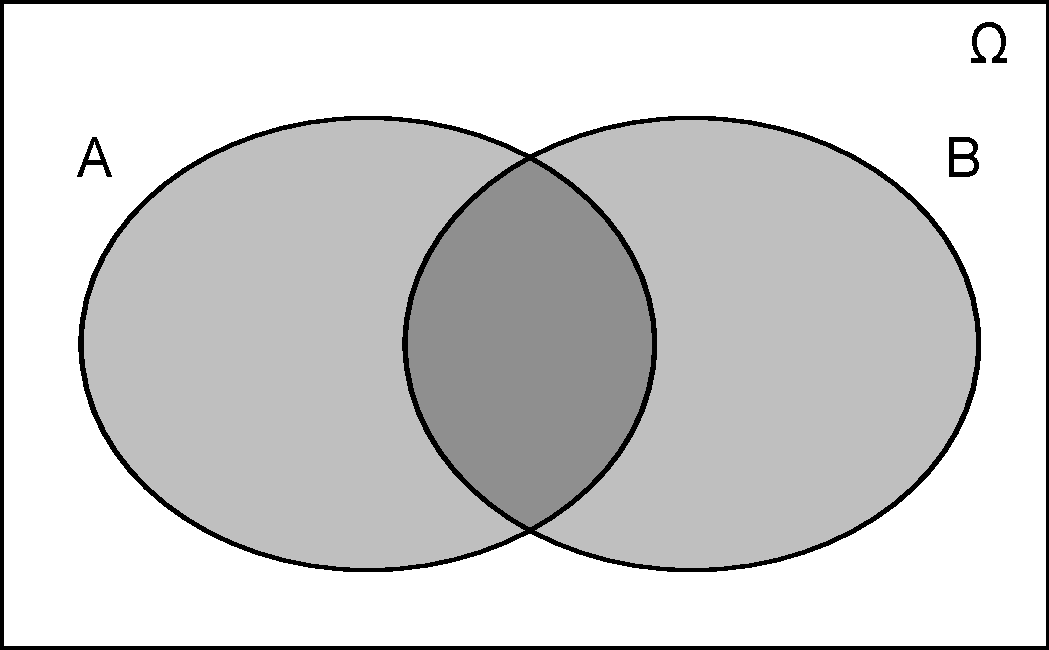
\includegraphics[width=7cm]{introdiscreteprobas/sets-union.pdf}
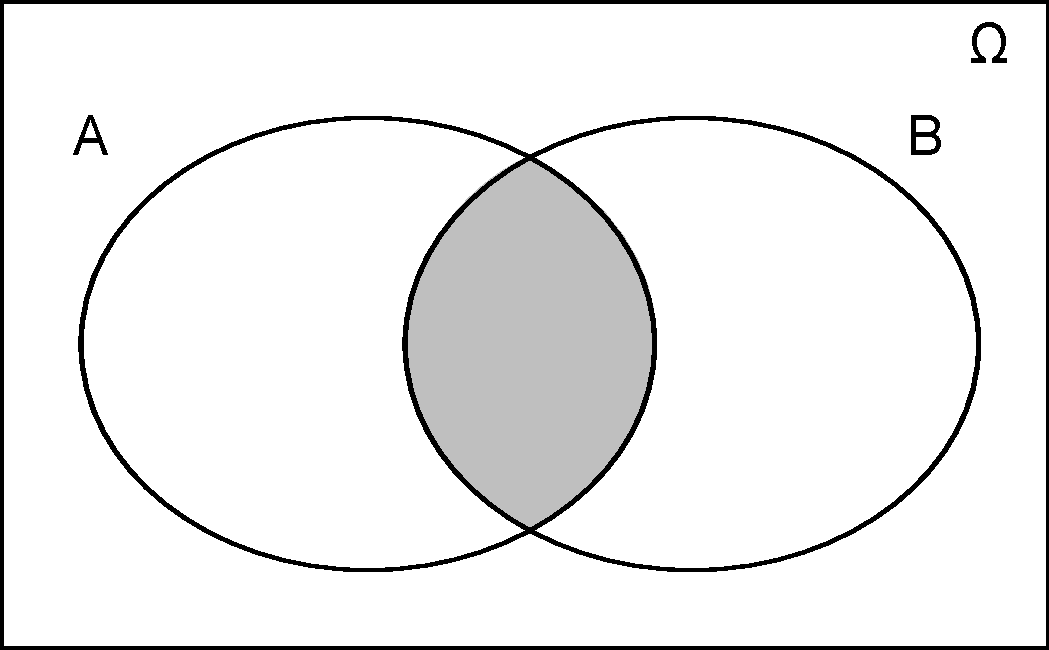
\includegraphics[width=7cm]{introdiscreteprobas/sets-intersection.pdf}
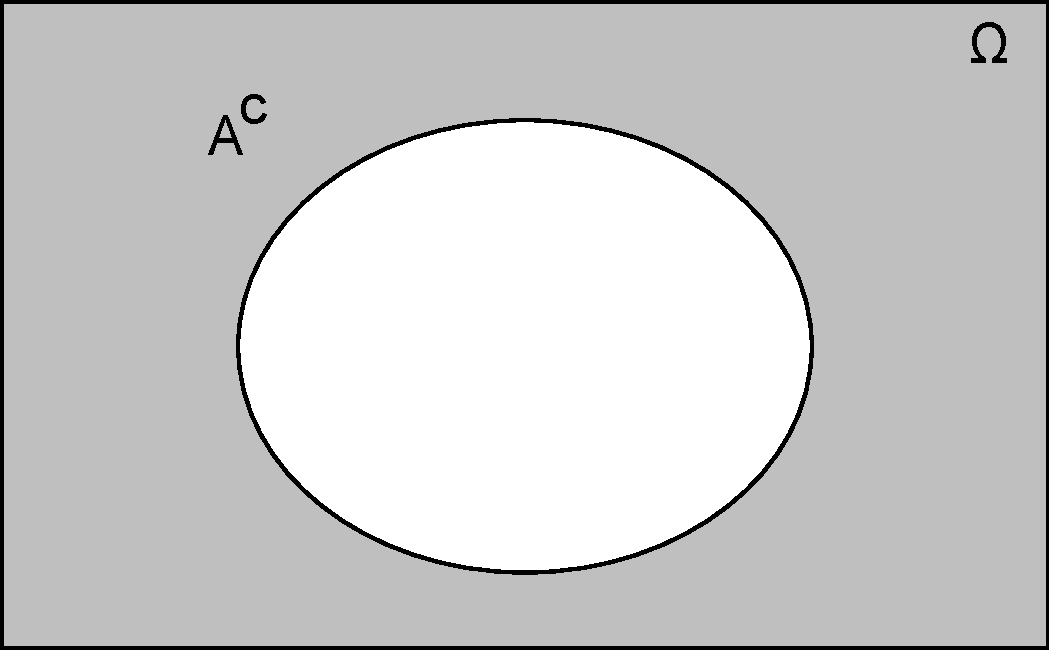
\includegraphics[width=7cm]{introdiscreteprobas/sets-complement.pdf}
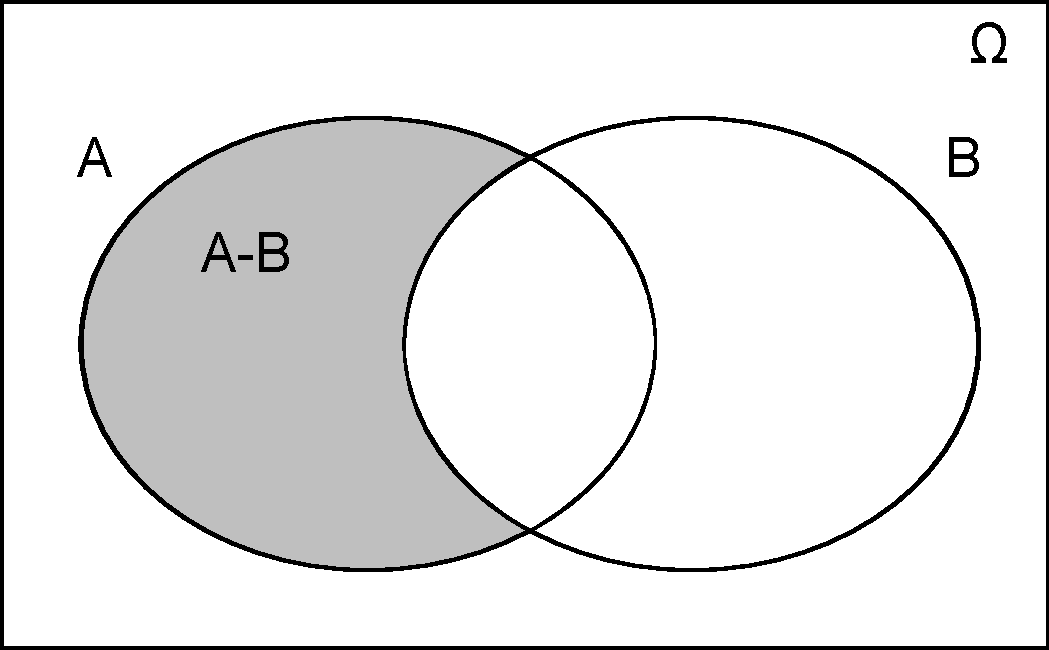
\includegraphics[width=7cm]{introdiscreteprobas/sets-difference.pdf}
\end{center}
\caption{Operations on sets -- Upper left, union: $A\cup B$, 
Upper right, intersection: $A\cap B$, Lower left, complement: $A^c$,
Lower right, difference: $A-B$}
\label{fig-introstats-operationsonsets}
\end{figure}

Two sets $A$ and $B$ are \emph{disjoints}, or \emph{mutually exclusive} 
if their intersection is empty, i.e. $A\cap B = \emptyset$.

In the following, we will use the fact that we can always decompose 
the union of two sets as the union of three disjoints subsets.
Indeed, assume that $A,B\subset \Omega$. 
We have
\begin{eqnarray}
A\cup B = (A-B) \cup (A\cap B) \cup (B-A),
\end{eqnarray}
where the sets $A-B$, $A\cap B$ and $B-A$ are disjoints.
This decomposition will be used several times in this chapter.

The cross product of two sets is the set
\begin{eqnarray}
A\times B = \left\{(x,y)\; / x \in A , y\in B\right\}.
\end{eqnarray}
Assume that $n$ is a positive integer.
The power set $A^n$ is the set
\begin{eqnarray}
A^n = \left\{(x_1,\ldots,x_n)\; / x_1,...,x_n \in A\right\}.
\end{eqnarray}

\begin{example}
\emph{(Die with 6 faces)}
\label{introstats-die6faces-sets}
Assume that a 6-face die is rolled once. The sample space for this experiment is
\begin{eqnarray}
\Omega=\left\{1,2,3,4,5,6\right\}.
\end{eqnarray}
The set of even numbers is $A=\left\{2,4,6\right\}$ and the 
set of odd numbers is $B=\left\{1,3,5\right\}$. Their 
intersection is empty, i.e. $A\cap B=\emptyset$ which proves that $A$ and $B$ 
are disjoints. Since their union is the whole sample space, i.e. $A\cup B=\Omega$,
these two sets are mutually complement, i.e. $A^c = B$ and $B^c = A$.
\end{example}

%%%%%%%%%%%%%%%%%%%%%%%%%%%%%%%%%%%%%%%%%%%%%%%%%%%%%%%%%%%%%%%%%%%%%%%%%%%%%%%%%%%%%%%
\subsection{Distribution function and probability}
A random event is an event which has a chance of happening, and 
the probability is a numerical measure of that chance.
What exactly is random is quite difficult to define.
In this section, we define the \emph{probability} associated 
with a distribution function, a concept that can be defined very precisely.

\index{event}
\index{outcome}
\index{sample space}
\index{random}
Assume that $\Omega$ is a set, called the \emph{sample space}. 
In this document, we will consider the case where the 
sample space is finite, i.e. the number of elements in $\Omega$ is finite.
Assume that we are performing \emph{random} trials, 
so that each trial is associated to one \emph{outcome} $x\in \Omega$.
Each subset $A$ of the sample space $\Omega$ is called an \emph{event}.
We say that event $A\cap B$ occurs if both the events $A$ and $B$ occur.
We say that event $A\cup B$ occurs if the event $A$ or the event $B$ occurs.

We will first define a \emph{distribution function} and then derive 
the \emph{probability} from there. The example of a 6-faces die will
serve as an example for these definitions.

\begin{definition}
\emph{(Distribution)}
\label{introstats-defdistrib}
A distribution function is a function $f:\Omega\rightarrow [0,1]$ which 
satisfies 
\begin{eqnarray}
0\leq f(x)\leq 1, \label{introstats-fin01}
\end{eqnarray}
for all $x\in\Omega$ and 
\begin{eqnarray}
\sum_{x\in\Omega} f(x)= 1 \label{introstats-sumfeq1}.
\end{eqnarray}
\end{definition}

\begin{example}
\emph{(Die with 6 faces)}
\label{introstats-die6faces}
Assume that a 6-face die is rolled once. The sample space for this experiment is
\begin{eqnarray}
\Omega=\left\{1,2,3,4,5,6\right\}.
\end{eqnarray}
Assume that the die is fair. This means that the probability 
of each of the six outcomes is the same, i.e. the distribution function is 
$f(x)=1/6$ for $x\in\Omega$, which satisfies the conditions of the definition 
\ref{introstats-defdistrib}.
\end{example}

\begin{definition}
\emph{(Probability)}
\label{introstats-defproba}
Assume that $f$ is a distribution function on the sample space $\Omega$.
For any event $A\subset \Omega$, the probability $P$ of $A$ is 
\begin{eqnarray}
P(A) = \sum_{x\in A} f(x) \label{introstats-probasumf}.
\end{eqnarray}
\end{definition}

\begin{example}
\emph{(Die with 6 faces)}
\label{introstats-die6faces2}
Assume that a 6-face die is rolled once so that the sample space for this experiment is
$\Omega=\left\{1,2,3,4,5,6\right\}$.
Assume that the distribution function is $f(x)=1/6$ for $x\in\Omega$.
The event 
\begin{eqnarray}
A=\left\{2,4,6\right\}
\end{eqnarray}
corresponds to the statement that the result of the roll is an even number.
From the definition \ref{introstats-defproba}, the probability of the 
event $A$ is 
\begin{eqnarray}
P(A)&=&f(2) + f(4) + f(6) \\
&=& \frac{1}{6} + \frac{1}{6} + \frac{1}{6} = \frac{1}{2}.
\end{eqnarray}
\end{example}

%If the events $A$ and $B$ are disjoints ,i.e. the intersection $A\cap B$ is empty, 
%then the even $\cup$ is replaced by $+$ so that $A\cap B = A+B$.

%%%%%%%%%%%%%%%%%%%%%%%%%%%%%%%%%%%%%%%%%%%%%%%%%%%%%%%%%%%%%%%%%%%%%%%%%%%%%%%%%%%%%%%
\subsection{Properties of discrete probabilities}
\label{introstats-probaproperties}
In this section, we present the properties that the probability $P(A)$ 
satisfies. We also derive some results for the probabilities of other 
events, such as unions of disjoints events.

The following theorem gives some elementary properties satisfied by a 
probability $P$.

\begin{proposition}
\emph{(Probability)}
\label{introstats-propoproba}
Assume that $\Omega$ is a sample space and that $f$ is a distribution
function on $\Omega$. Assume that $P$ is the probability associated with
$f$. 
The probability of the event $\Omega$ is one, i.e. 
\begin{eqnarray}
P(\Omega) = 1 \label{introstats-pomegaone}.
\end{eqnarray}
The probability of the empty set is zero, i.e. 
\begin{eqnarray}
P(\emptyset) = 0 \label{introstats-pemptyzero}.
\end{eqnarray}
Assume that $A$ and $B$ are two subsets of $\Omega$. 
If $A\subset B$, then
\begin{eqnarray}
P(A) \leq P(B). \label{introstats-asubsetb}
\end{eqnarray}
For any event $A\subset \Omega$, we have 
\begin{eqnarray}
0\leq P(A) \leq 1.  \label{introstats-pzerone}
\end{eqnarray}
\end{proposition}

\begin{proof}
The equality \ref{introstats-pomegaone} derives directly from the definition
\ref{introstats-sumfeq1} of a distribution function,
i.e. $P(\Omega) = \sum_{x\in\Omega} f(x) = 1$.
The equality \ref{introstats-pemptyzero} derives directly from \ref{introstats-sumfeq1}.

Assume that $A$ and $B$ are two subsets of $\Omega$ so that $A\subset B$. 
Since a probability is the sum of positive terms, we have
\begin{eqnarray}
P(A)= \sum_{x\in A} f(x) \leq \sum_{x\in B} f(x) = P(B)
\end{eqnarray}
which proves the inequality \ref{introstats-asubsetb}.

The inequalities \ref{introstats-pzerone} derive directly from the definition
of a probability \ref{introstats-probasumf}.
First, the probability $P$ is positive since \ref{introstats-fin01} states that $f$ is 
positive. Second, the probability $P$ of an event $A$ is lower than 1, since 
$P(A)= \sum_{x\in A} f(x) \leq \sum_{x\in\Omega} f(x) = P(\Omega)= 1$, which concludes the proof.
\end{proof}

\begin{proposition}
\emph{(Probability of two disjoint subsets)}
\label{introstats-propopdisjoint}
Assume that $\Omega$ is a sample space and that $f$ is a distribution
function on $\Omega$. Assume that $P$ is the probability associated with
$f$.

Let $A$ and $B$ be two disjoints subsets of $\Omega$, then 
\begin{eqnarray}
P(A \cup B ) = P(A) + P(B)\label{introstats-pdisjointssum}.
\end{eqnarray}
\end{proposition}

The figure \ref{fig-introstats-disjointsets} presents the situation
of two disjoints sets $A$ and $B$. Since the two sets have no 
intersection, it suffices to add the probabilities associated 
with each event.

\begin{figure}
\begin{center}
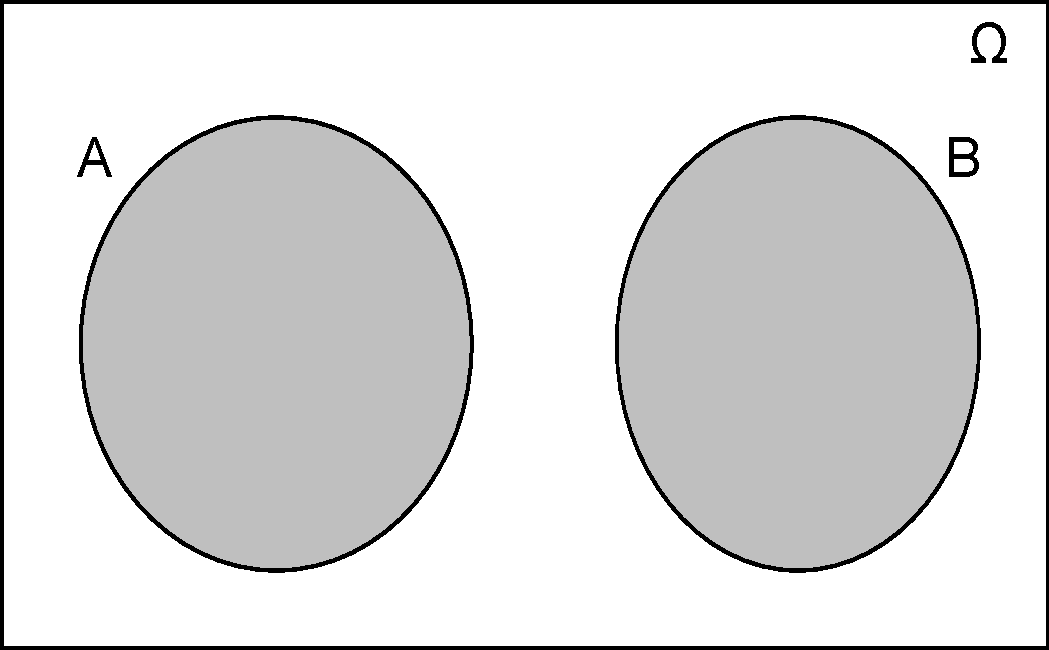
\includegraphics[width=7cm]{introdiscreteprobas/sets-disjointunion.pdf}
\end{center}
\caption{Two disjoint sets.}
\label{fig-introstats-disjointsets}
\end{figure}

\begin{proof}
Assume that $A$ and $B$ be two disjoints subsets of $\Omega$.
We can decompose $A\cup B$ as $A\cup B = (A-B) \cup (A\cap B) \cup (B-A)$, so that 
\begin{eqnarray}
P(A \cup B ) &=& \sum_{x\in A\cup B} f(x) \\
&=& \sum_{x\in A- B} f(x) + \sum_{x\in A\cap B} f(x) + \sum_{x\in B- A} f(x).
\end{eqnarray}
But $A$ and $B$ are disjoints, so that $A-B = A$, $A\cap B = \emptyset$
and $B-A = B$. Therefore,
\begin{eqnarray}
P(A \cup B ) &=& \sum_{x\in A} f(x) + \sum_{x\in B} f(x)\\
&=&P(A) + P(B),
\end{eqnarray}
which concludes the proof. 
\end{proof}

Notice that the equality \ref{introstats-pdisjointssum} can be generalized immediately
to a sequence of disjoints events.

\begin{proposition}
\emph{(Probability of disjoints subsets)}
\label{introstats-sequencedisjoint}
Assume that $\Omega$ is a sample space and that $f$ is a distribution
function on $\Omega$. Assume that $P$ is the probability associated with
$f$.

For any disjoints events $A_1, A_2, \ldots , A_k\subset \Omega$ with $k\geq 0$, we have
\begin{eqnarray}
P\left(A_1 \cup A_2 \cup \ldots \cup A_k \right) = 
P(A_1) + P(A_2) + \ldots + P(A_k)\label{introstats-pdisjointssumk}.
\end{eqnarray}
\end{proposition}

\begin{proof}
For example, we can use the proposition \ref{introstats-propopdisjoint} 
to state the proof by induction on the number of events.
\end{proof}

\begin{example}
\emph{(Die with 6 faces)}
\label{introstats-die6faces3}
Assume that a 6-face die is rolled once so that the sample space for this experiment is
$\Omega=\left\{1,2,3,4,5,6\right\}$.
Assume that the distribution function is $f(x)=1/6$ for $x\in\Omega$.
The event $A=\left\{1,2,3\right\}$ corresponds to the numbers lower or equal to 3.
The probability of this event is $P(A)= \frac{1}{2}$. 
The event $B=\left\{5,6\right\}$ corresponds to the numbers greater than 5.
The probability of this event is $P(B)=\frac{1}{3}$.
The two events are disjoints, so that the proposition 
\ref{introstats-sequencedisjoint} can be applied which proves that $P(A\cup B) = \frac{5}{6}$.
\end{example}

\begin{proposition}
\emph{(Probability of the complementary event)}
\label{introstats-propocomplem}
Assume that $\Omega$ is a sample space and that $f$ is a distribution
function on $\Omega$. Assume that $P$ is the probability associated with
$f$.

For all subset $A$ of $\Omega$, 
\begin{eqnarray}
P(A) + P(A^c) = 1. \label{introstats-theoremcomplem}
\end{eqnarray}
\end{proposition}

\begin{proof}
We have $\Omega = A\cup A^c$, where the sets $A$ and $A^c$ are disjoints. Therefore, from 
proposition \ref{introstats-propopdisjoint}, we have 
\begin{eqnarray}
P(\Omega) = P(A) + P(A^c),
\end{eqnarray}
where $P(\Omega) = 1$, which concludes the proof.
\end{proof}

\begin{example}
\emph{(Die with 6 faces)}
\label{introstats-die6faces4}
Assume that a 6-face die is rolled once so that the sample space for this experiment is
$\Omega=\left\{1,2,3,4,5,6\right\}$.
Assume that the distribution function is $f(x)=1/6$ for $x\in\Omega$.
The event $A=\left\{2,4,6\right\}$ corresponds to the statement that the result of the roll is an even number.
The probability of this event is $P(A)= \frac{1}{2}$. 
The complementary event is the event of an odd number, i.e. $A^c = \left\{1,3,5\right\}$.
By proposition \ref{introstats-propocomplem}, the probability of an odd number is 
$P(A^c) = 1 - P(A) = 1 - \frac{1}{2} = \frac{1}{2}$.
\end{example}

The following equality gives the relationship between the probability
of the union of two events in terms of the individual probabilities and the 
probability of the intersection. 

\begin{proposition}
\emph{(Probability of the union)}
\label{introstats-propounion}
Assume that $\Omega$ is a sample space and that $f$ is a distribution
function on $\Omega$. Assume that $A$ and $B$ are two subsets of $\Omega$, not 
necessarily disjoints. We have:
\begin{eqnarray}
P(A\cup B) = P(A) + P(B) - P(A\cap B).
\end{eqnarray}
\end{proposition}

The figure \ref{fig-introstats-jointsets} presents the situation 
where two sets $A$ and $B$ have a non empty intersection.
When we add the probabilities of the two events $A$ and $B$, the 
intersection is added twice. This is why it must be removed by 
subtraction.

\begin{figure}
\begin{center}
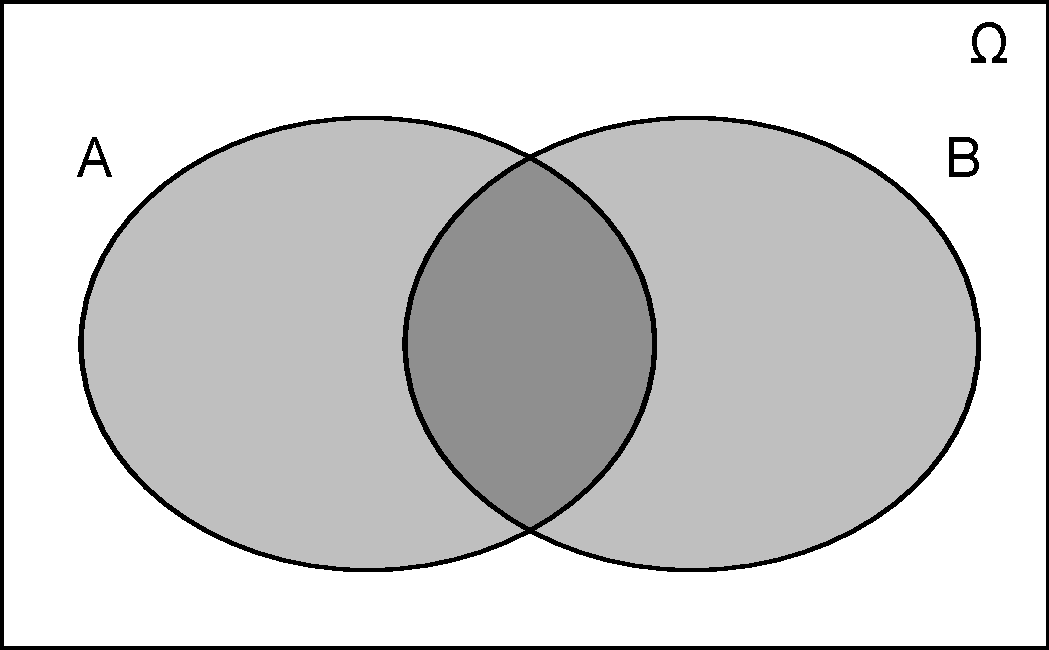
\includegraphics[width=7cm]{introdiscreteprobas/sets-union.pdf}
\end{center}
\caption{Two sets with a non empty intersection.}
\label{fig-introstats-jointsets}
\end{figure}

\begin{proof}
Assume that $A$ and $B$ are two subsets of $\Omega$.
The proof is based on the analysis of Venn's diagram presented in
figure \ref{fig-introstats-operationsonsets}. The idea of the 
proof is to compute the probability $P(A\cup B)$, by making disjoints sets on which the 
equality \ref{introstats-pdisjointssum} can be applied.
We can decompose the union of the two set $A$ and $B$ as the 
union of disjoints sets:
\begin{eqnarray}
A\cup B = (A-B)\cup(A\cap B)\cup(B-A).
\end{eqnarray}
The equality \ref{introstats-pdisjointssum} leads to 
\begin{eqnarray}
\label{introstats-proofaunionb1}
P(A\cup B) = P(A-B) + P(A\cap B) + P(B-A).
\end{eqnarray}
The next part of the proof is based on the computation of 
$P(A-B)$ and $P(B-A)$.
We can decompose the set $A$ as the union of disjoints 
sets
\begin{eqnarray}
A = (A - B)\cup (A\cap B),
\end{eqnarray}
which leads to $P(A) = P(A - B) + P(A\cap B)$,
which can be written as 
\begin{eqnarray}
\label{introstats-proofaunionb2}
P(A - B) = P(A) - P(A\cap B).
\end{eqnarray}
Similarly, we can prove that 
\begin{eqnarray}
\label{introstats-proofaunionb3}
P(B - A) = P(B) - P(B\cap A).
\end{eqnarray}
By plugging the two equalities \ref{introstats-proofaunionb2}
and \ref{introstats-proofaunionb3} into \ref{introstats-proofaunionb1},
we find 
\begin{eqnarray}
P(A\cup B) = P(A) - P(A\cap B) + P(A\cap B) + P(B) - P(B\cap A),
\end{eqnarray}
which simplifies into
\begin{eqnarray}
P(A\cup B) = P(A) + P(B) - P(B\cap A),
\end{eqnarray}
and concludes the proof.
\end{proof}


\begin{example}
\emph{(Disease)}
\label{introstats-probabactvirus}
Assume that the probability of infections can be bacterial (B), viral (V) or 
both ($B\cap V$). This implies that $B\cup V=\Omega$ but the two events 
are not disjoints, i.e. $B\cap V \neq \emptyset$. Assume that $P(B)=0.7$ and $P(V)=0.4$.
What is the probability of having both types of infections ?
The probability of having both infections is $P(B\cap V)$. 
From proposition \ref{introstats-propounion}, we have $P(B\cup V) = P(B) + P(V) - P(B\cap V)$,
which leads to $P(B\cap V) = P(B) + P(V) - P(B\cup V)$.
We finally get $P(B\cap V) = 0.1$.
This example is presented in \cite{lectureIntroToProbastats}.
\end{example}

%%%%%%%%%%%%%%%%%%%%%%%%%%%%%%%%%%%%%%%%%%%%%%%%%%%%%%%%%%%%%%%%%%%%%%%%%%%%%%%%%%%%%%%
\subsection{Uniform distribution}

In this section, we describe the particular situation
where the distribution function is \emph{uniform}.
\index{uniform}

\index{uniform}
\begin{definition}
\emph{(Uniform distribution)}
\label{introstats-unifdistrib}
Assume that $\Omega$ is a finite sample space.
The uniform distribution function is 
\begin{eqnarray}
\label{introstats-eq-unifdistrib}
f(x) = \frac{1}{\#(\Omega)},
\end{eqnarray}
for all $x\in\Omega$.
\end{definition}

\begin{proposition}
\emph{(Probability with uniform distribution)}
\label{introstats-probauniform}
Assume that $\Omega$ is a finite sample space and 
that $f$ is a uniform distribution function.
Then the probability of the event $A\subset \Omega$ is 
\begin{eqnarray}
P(A) = \frac{\#(A)}{\#(\Omega)}.
\end{eqnarray}
\end{proposition}

\begin{proof}
When the distribution function is uniform, the definition 
\ref{introstats-defproba} implies that 
\begin{eqnarray}
P(A) &=& \sum_{x\in A} f(x) = \sum_{x\in A} \frac{1}{\#(\Omega)} \\
&=& \frac{\#(A)}{\#(\Omega)},
\end{eqnarray}
which concludes the proof. 
\end{proof}

\begin{example}
\emph{(Die with 6 faces)}
\label{introstats-die6faces5}
\index{fair die}
Assume that a 6-face die is rolled once so that the sample space for this experiment is
$\Omega=\left\{1,2,3,4,5,6\right\}$.
In the previous analysis of this example, we have assumed that the distribution 
function is $f(x)=1/6$ for $x\in\Omega$.
This is consistent with definition \ref{introstats-unifdistrib}, since $\#(\Omega) = 6$.
Such a die is a \emph{fair} die, meaning that all faces have the same probability. 
The event $A=\left\{2,4,6\right\}$ corresponds to the statement that the result of the roll is an even number.
The number of outcomes in this event is $\#(A)=3$.
From proposition \ref{introstats-probauniform}, the probability of this event is $P(A)= \frac{1}{2}$. 
\end{example}

%%%%%%%%%%%%%%%%%%%%%%%%%%%%%%%%%%%%%%%%%%%%%%%%%%%%%%%%%%%%%%%%%%%%%%%%%%%%%%%%%%%%%%%
\subsection{Conditional probability}
\index{conditional!probability}

In this section, we define the conditional distribution function and
the conditional probability.
We analyze this definition in the particular situation of the 
uniform distribution.

In some situations, we want to consider the probability of 
an event $A$ given that an event $B$ has occurred. 
In this case, we consider the set $B$ as a new sample space, 
and update the definition of the distribution function accordingly.

\index{conditional!distribution function}
\begin{definition}
\emph{(Conditional distribution function)}
\label{introstats-conddistribution}
Assume that $\Omega$ is a sample space and that $f$ is a distribution
function on $\Omega$.  
Assume that $A$ is a subset of $\Omega$ with $P(A)=\sum_{x\in A} f(x)>0$.
The function $f(x|A)$ defined by
\begin{eqnarray}
\label{introstats-eq-conddistrib}
f(x|A) = \left\{
\begin{array}{l}
\frac{f(x)}{\sum_{x\in A} f(x)}, \textrm{ if }  x\in A,\\
0, \textrm{ if } x\notin A,
\end{array}
\right.
\end{eqnarray}
is the conditional distribution function of $x$ given A.
\end{definition}

The figure \ref{fig-introstats-onesetA} presents the situation where 
an event $A$ is considered for a conditionnal distribution.
The distribution function $f(x)$ is with respect to the sample 
space $\Omega$ while the conditionnal distribution function $f(x|A)$ 
is with respect to the set $A$.

\begin{figure}
\begin{center}
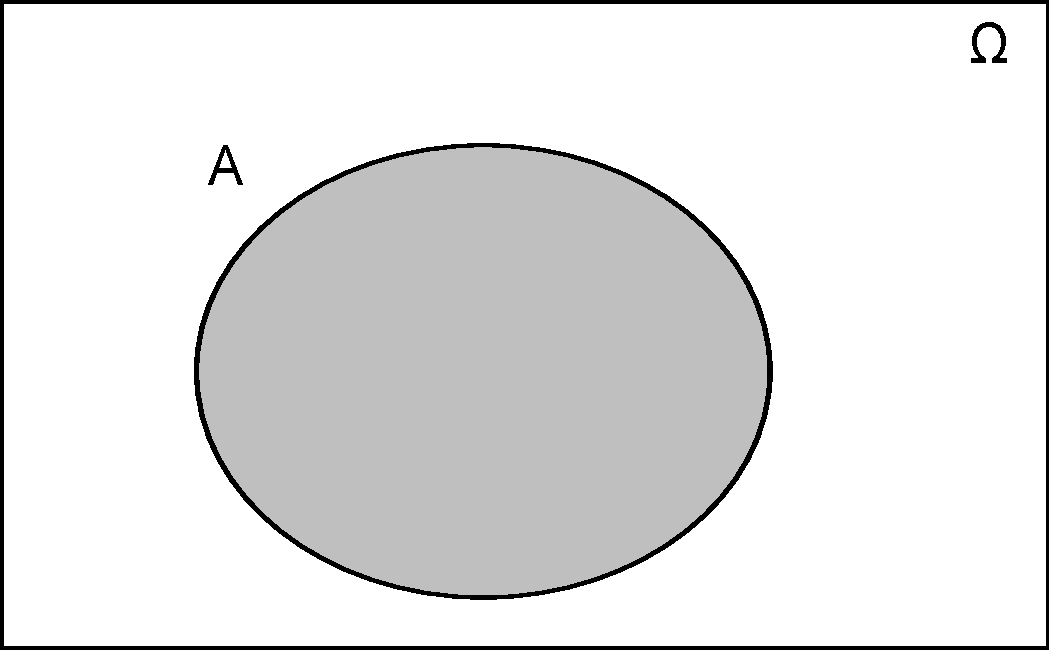
\includegraphics[width=7cm]{introdiscreteprobas/sets-setA.pdf}
\end{center}
\caption{A set $A$, subset of the sample space $\Omega$.}
\label{fig-introstats-onesetA}
\end{figure}

\begin{proof}
What is to be proved in this proposition is that the function 
$f(x|A)$ is a distribution function.
Let us prove that the function $f(x|A)$ satisfies 
the equality 
\begin{eqnarray}
\label{introstats-eq-conddistribproof1}
\sum_{x\in \Omega} f(x|A) = 1.
\end{eqnarray}
Indeed, we have 
\begin{eqnarray}
\sum_{x\in \Omega} f(x|A) &=& \sum_{x\in A} f(x|A) + \sum_{x\notin A} f(x|A)\\
&=&\sum_{x\in A} \frac{f(x)}{\sum_{x\in A} f(x)}\\
&=&1,\\
\end{eqnarray}
which concludes the proof.
\end{proof}

This leads us to the following definition of the 
conditional probability of an event $A$ given an event $B$.

\begin{proposition}
\emph{(Conditional probability)}
\label{introstats-condproba}
Assume that $\Omega$ is a finite sample space and $A$ and $B$ are two 
subsets of $\Omega$. Assume that $P(B)>0$.
The conditional probability of the event $A$ given the event $B$ is  
\begin{eqnarray}
\label{introstats-eq-pabcond}
P(A|B) = \frac{P(A\cap B)}{P(B)}.
\end{eqnarray}
\end{proposition}

The figure \ref{fig-introstats-setcondproba} presents the situation where 
we consider the event $A|B$.
The probability $P(A)$ is with respect to $\Omega$ while the 
probability $P(A|B)$ is with respect to $B$.

\begin{figure}
\begin{center}
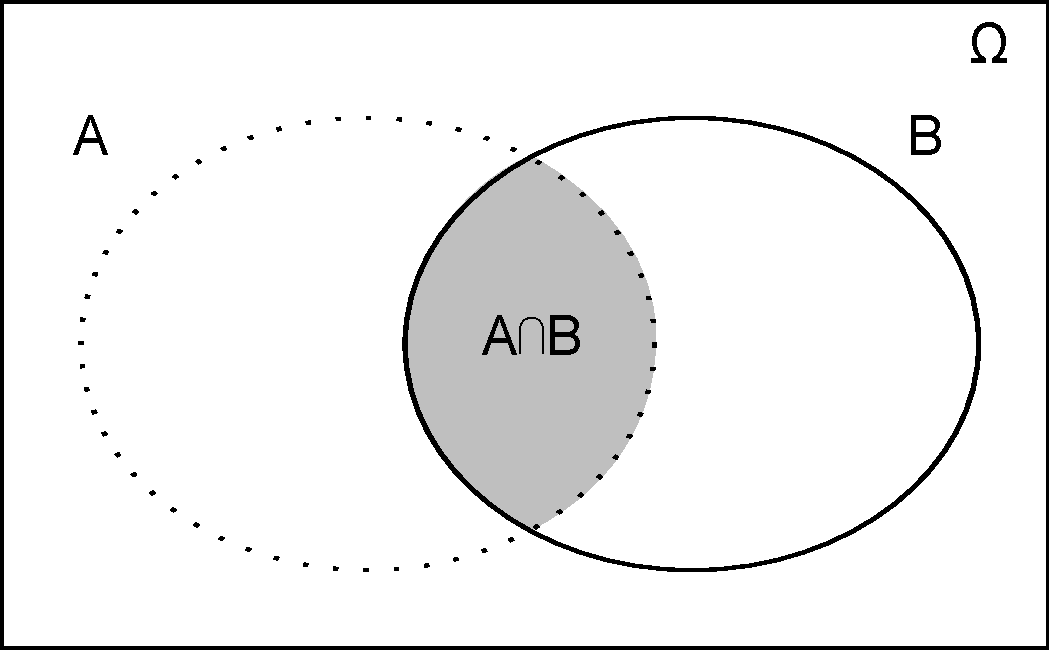
\includegraphics[width=7cm]{introdiscreteprobas/sets-condproba.pdf}
\end{center}
\caption{The conditionnal probability $P(A|B)$ measure the probability of  
the set $A\cap B$ with respect to the set $B$.}
\label{fig-introstats-setcondproba}
\end{figure}

\begin{proof}
Assume that $A$ and $B$ are subsets of the sample space $\Omega$.
The conditional distribution function $f(x|B)$ allows 
us to compute the probability of the event $A$ given the event $B$.
Indeed, we have
\begin{eqnarray}
P(A|B) 
&=& \sum_{x\in A} f(x|B)\\
&=& \sum_{x\in A\cap B} f(x|B)
\end{eqnarray}
since $f(x|B)= 0$ if $x\notin B$.
Hence,
\begin{eqnarray}
P(A|B) &=& \sum_{x\in A\cap B} \frac{f(x)}{\sum_{x\in B} f(x)} \\
&=&  \frac{\sum_{x\in A\cap B} f(x)}{\sum_{x\in B} f(x)} \\
&=&  \frac{P(A\cap B)}{P(B)}.
\end{eqnarray}
The previous equality is well defined since $P(B)>0$.
\end{proof}

This definition can be analyzed in the particular case 
where the distribution function is uniform. 
Assume that $\#(\Omega)$ is the size of the sample space and $\#(A)$ (resp. $\#(B)$ and 
$\#(A\cap B)$) is the number of elements of $A$ (resp. of $B$ and 
$A\cap B$). The conditional probability $P(A|B)$ is 
\begin{eqnarray}
P(A|B) = \frac{\#(A\cap B)}{\#(B)}.
\end{eqnarray}
We notice that
\begin{eqnarray}
\frac{\#(B)}{\#(\Omega)} \frac{\#(A\cap B)}{\#(B)} = \frac{\#(A\cap B)}{\#(\Omega)},
\end{eqnarray}
for all $A,B\subset \Omega$. This leads to the equality 
\begin{eqnarray}
P(B) P(A|B) = P(A\cap B),
\end{eqnarray}
for all $A,B\subset \Omega$. The previous equation could have been directly found based on the 
equation \ref{introstats-eq-pabcond}.

The following example is given in \cite{introprobasGrinsteadSnell},
in section 4.1, "Discrete conditional Probability".

\begin{example}
Grinstead and Snell \cite{introprobasGrinsteadSnell} present a table 
which presents the number of survivors at single years of age.
This table gathers data compiled in the USA in 1990.
The first line counts 100,000 born alive persons, with decreasing 
values when the age is increasing. This table allows to 
see that 89.8 \% in a population of 100,000 females can expect to 
live to age 60, while 57.0 \% can expect to live to age 80. Given
that a women is 60, what is the probability that she lives 
to age 80 ?

Let us denote by $A=\{a\geq 60\}$ the event that a woman lives to age 60, 
and let us denote by $B=\{a\geq 80\}$ the event that a woman lives to age 80.
We want to compute the conditionnal probability $P(\{a\geq 80\} | \{a\geq 60\})$. 
By the proposition \ref{introstats-condproba}, we have
\begin{eqnarray}
P(\{a\geq 80\} | \{a\geq 60\}) 
&=& \frac{P(\{a\geq 60\}\cap \{a\geq 80\})}{P(\{a\geq 60\})}\\
&=& \frac{P(\{a\geq 80\})}{P(\{a\geq 60\})}\\
&=& \frac{0.570}{0.898}\\
&=&0.635,
\end{eqnarray}
with 3 significant digits.
In other words, a women who is already 60, has 63.5 \% of chance 
to live to 80.
\end{example}

%%%%%%%%%%%%%%%%%%%%%%%%%%%%%%%%%%%%%%%%%%%%%%%%%%%%%%%%%%%%%%%%%%%%%%%%%%%%%%%%%%%%%%%

\section{Combinatorics}
\label{introstats-chap-combinatorics}

\index{combinatorics}
In this section, we present several tools which allow to compute 
probabilities of discrete events. One powerful analysis tool is 
the tree diagram, which is presented in the first part of this section.
Then, we detail permutations and combinations numbers,
which allow to solve many probability problems.

%%%%%%%%%%%%%%%%%%%%%%%%%%%%%%%%%%%%%%%%%%%%%%%%%%%%%%%%%%%%%%%%%%%%%%%%%%%%%%%%%%%%%%%
\subsection{Tree diagrams}

\index{tree diagram}
In this section, we present the general method which allows to count 
the total number of ways that a task can be performed. We illustrate that
method with tree diagrams.

Assume that a task is carried out in a sequence of $n$ steps. 
The first step can be performed by making one choice among $m_1$ possible choices.
Similarly, there are $m_2$ possible ways to perform the second step, and so forth.
The total number of ways to perform the complete sequence can be performed in
$n=m_1 m_2 \ldots m_n$ different ways.

To illustrate the sequence of steps, the associated tree can be drawn. 
An example of such a tree diagram is given in the figure \ref{fig-introstats-tree-diagram}.
Each node in the tree corresponds to one step in the sequence. 
The number of children of a parent node is equal to the number of 
possible choices for the step. At the bottom of the tree, there are $N$ leafs,
where each path, i.e. each sequence of nodes from the root to the leaf, 
corresponds to a particular sequence of choices. 

\begin{figure}
\begin{center}
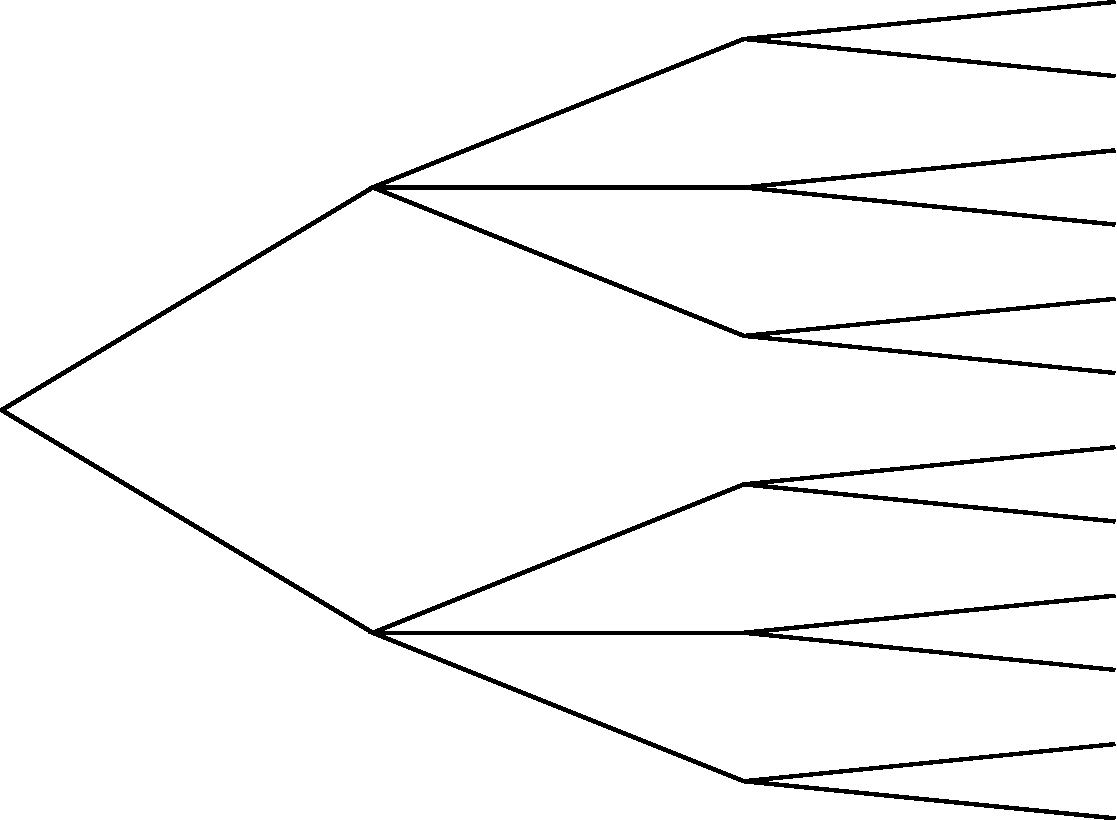
\includegraphics[width=7cm]{introdiscreteprobas/tree-diagram.pdf}
\end{center}
\caption{Tree diagram - The task is made with 3 steps. There are 2 choices for the 
step \#1, 3 choices for step \#2 and 2 choices for step \#3. The total number of 
ways to perform the full sequence of steps is $n=2\cdot 3\cdot 2 = 12$.}
\label{fig-introstats-tree-diagram}
\end{figure}

We can think of the tree as representing a random experiment, where 
the final state is the outcome of the experiment. In this context, each 
choice is performed at random, depending on the probability 
associated with each branch. We will review tree diagrams throughout
this section and especially in the section devoted to Bernoulli 
trials.

%%%%%%%%%%%%%%%%%%%%%%%%%%%%%%%%%%%%%%%%%%%%%%%%%%%%%%%%%%%%%%%%%%%%%%%%%%%%%%%%%%%%%%%
\subsection{Permutations}

In this section, we present permutations, which are ordered subsets
of a given set.

\index{permutation}
\begin{definition}
(\emph{Permutation})
Assume that $A$ is a finite set. A permutation of $A$ is a one-to-one mapping
of $A$ onto itself.
\end{definition}

Without loss of generality, we can assume that the finite set $A$ can be
ordered and numbered from 1 to $n=\#(A)$, so that we can 
write $A=\{1,2,\ldots,n\}$. To define a particular permutation, one 
can write a matrix with 2 rows and $n$ columns which represents the 
mapping. One example of a permutation on the set $A=\{a_1,a_2,a_3,a_4\}$ is 
\begin{eqnarray}
\sigma = 
\left(
\begin{array}{cccc}
1 & 2 & 3 & 4\\
2 & 1 & 4 & 3\\
\end{array}
\right),
\end{eqnarray}
which signifies that the mapping is:
\begin{itemize}
\item $a_1\rightarrow a_2$, 
\item $a_2\rightarrow a_1$, 
\item $a_3\rightarrow a_4$, 
\item $a_3\rightarrow a_4$.
\end{itemize}
Since the first row is always the same, there is no additional information
provided by this row. This is why the permutation can be written by uniquely
defining the second row. This way, the previous mapping can be written as
\begin{eqnarray}
\sigma = 
\left(
\begin{array}{cccc}
2 & 1 & 4 & 3\\
\end{array}
\right).
\end{eqnarray}

We can try to count the number of possible permutations of a given set $A$
with $n$ elements. 

The tree diagram associated with the computation of the number of 
permutations for $n=3$ is presented in figure \ref{fig-introstats-treediag-permutation}.
In the first step, we decide which number to place at index 1. For this index,
we have 3 possibilities, that is, the numbers 1, 2 and 3. In the second
step, we decide which number to place at index 2. At this index, we have 
2 possibilities left, where the exact numbers depend on the branch.
In the third step, we decide which number to place at index 3. At this last index,
we only have one number left.

\begin{figure}
\begin{center}
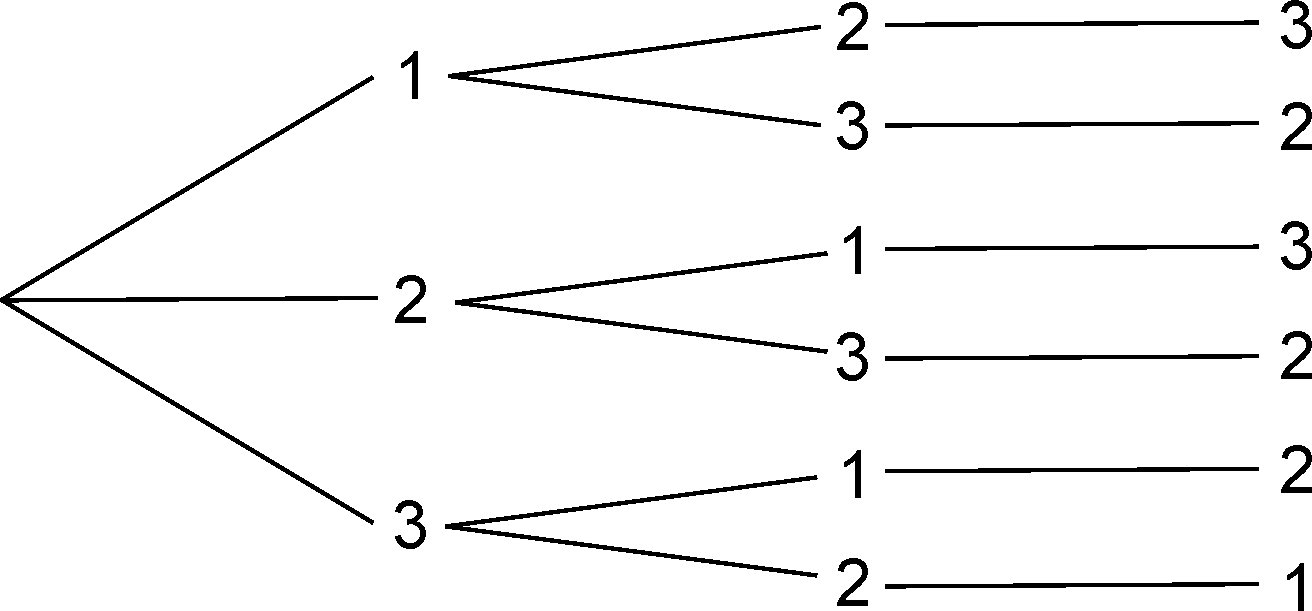
\includegraphics[width=7cm]{introdiscreteprobas/tree-permutation.pdf}
\end{center}
\caption{Tree diagram for the computation of permutations of the set $A=\{1,2,3\}$.}
\label{fig-introstats-treediag-permutation}
\end{figure}

This leads to the following proposition, which defines 
the factorial function.

\index{factorial}
\begin{proposition}
(\emph{Factorial})
\label{propo-factorial}
The number of permutations of a set $A$ of $n$ elements is 
the factorial of $n$ defined by 
\begin{eqnarray}
n! = n \cdot  (n-1) \ldots 2\cdot  1. \label{propo-factorial1}
\end{eqnarray}
\end{proposition}

\begin{proof} \textit{\#1}
Let us pick an element to place at index 1. There are $n$ elements in the set, leading to 
$n$ possible choices. For the element at index 2, there are $n-1$ elements left in the set. 
For the element at index $n$, there is only 1 element left. The total number of permutations is 
therefore $n\cdot (n-1) \ldots 2\cdot 1$, which concludes the proof.
\end{proof}

\begin{proof} \textit{\#2}
The element at index 1 can be located at indexes $1, 2, \ldots, n$ so that there are 
$n$ ways to set the element \#1. Once the element at index 1 is placed, there are $n-1$ 
ways to set the element at index 2. The last element at index $n$ can only be set at the remaining
index. The total number of permutations is therefore $n\cdot (n-1) \ldots 2\cdot 1$,
which concludes the proof. 
\end{proof}

When $n=0$, it seems that we cannot define the number $0!$.
For reasons which will be clearer when we will introduce the gamma 
function, it is convenient to define $0!$ as equal to one:
\begin{eqnarray}
0! = 1.
\end{eqnarray}

\begin{example}
Let us compute the number of permutations of the set $A=\{1,2,3\}$.
By the equation \ref{propo-factorial1}, we have $6!=3\cdot 2\cdot 1 = 6$ 
permutations of the set $A$. These permutations are:
\begin{eqnarray}
\begin{array}{ccc}
(1 &     2 &     3) \\
(1 &     3 &     2) \\
(2 &     1 &     3) \\
(2 &     3 &     1) \\
(3 &     1 &     2) \\
(3 &     2 &     1) \\
\end{array}
\end{eqnarray}
The previous permutations can also be directly read from the 
tree diagram \ref{fig-introstats-treediag-permutation}, from the root of the 
tree to each of the 6 leafs.
\end{example}

In some situations, all the elements in the set $A$ are not involved in the 
permutation. Assume that $j$ is a positive integer, so that $0\leq j\leq n$.
A $j$-permutation is a permutation of a subset of $j$ elements in $A$.
The general counting method used for the previous proposition allows 
to count the total number of $j$-permutations of a given set $A$.

\begin{proposition}
(\emph{$j$-permutations})
\label{propo-permutation}
Assume that $j$ is a positive integer. 
The number of $j$-permutations of a set $A$ of $n$ elements is 
\begin{eqnarray}
(n)_j = n \cdot  (n-1)  \ldots  (n-j+1). \label{propo-permutation1}
\end{eqnarray}
\end{proposition}

\begin{proof}
The element at index 1 can be located at indexes $1, 2, \ldots, n$ so that there are 
$n$ ways to set the element at index 1. Once element at index 1 is placed, there are $n-1$ 
ways to set the element at index 2. The element at index $j$ can only be set at the remaining
$n-j+1$ indexes. 
The total number of $j$-permutations is therefore $n\cdot (n-1) \ldots (n-j+1)$,
which concludes the proof. 
\end{proof}

Notice that the number of $j$-permutations of $n$ elements and the factorial of $n$
are equal when $j=n$. Indeed, we have
\begin{eqnarray}
(n)_n = n \cdot  (n-1)  \ldots  (n-n+1) = n!.
\end{eqnarray}
On the other hand, the number of $0$-permutations of $n$ elements 
can be defined to be equal to 1:
\begin{eqnarray}
(n)_0 = 1.
\end{eqnarray}

\begin{example}
Let us compute the number of 2-permutations of the set $A=\{1,2,3,4\}$.
By the equation \ref{propo-permutation1}, we have $(4)_2=4\cdot 3 = 12$ 
permutations of the set $A$. These permutations are:
\begin{eqnarray}
\begin{array}{cc}
(1 &     2 ) \\
(1 &     3 ) \\
(1 &     4 ) \\
\end{array}
\qquad 
\begin{array}{cc}
(2 &     1 ) \\
(2 &     3 ) \\
(2 &     4 ) \\
\end{array}
\qquad 
\begin{array}{cc}
(3 &     1 ) \\
(3 &     2 ) \\
(3 &     4 ) \\
\end{array}
\qquad
\begin{array}{cc}
(4 &     1 ) \\
(4 &     2 ) \\
(4 &     3 ) \\
\end{array}
\end{eqnarray}
We can check that the number of 2-permutations in a set of 4 elements is $(4)_2=12$
which is stricly lower that the number of permutations $4!=24$. 
\end{example}

%%%%%%%%%%%%%%%%%%%%%%%%%%%%%%%%%%%%%%%%%%%%%%%%%%%%%%%%%%%%%%%%%%%%%%%%%%%%%%%%%%%%%%%

\subsection{The gamma function}
\label{section-gammafun}

\index{gamma}
In this section, we present the gamma function which is 
closely related to the factorial function.
The gamma function was first introduced by the Swiss mathematician
Leonard Euler in his goal to generalize the factorial to non
integer values\cite{SebahGourdon2002}.
Efficient implementations of the factorial function are based 
on the gamma function and this is why this functions 
will be analyzed in detail. The practical computation 
of the factorial function will be analyzed in the next section.

\begin{definition}
(\emph{Gamma function})
\label{section-defgammafun}
Let $x$ be a real with $x>0$. The gamma function is defined by 
\begin{eqnarray}
\Gamma(x) = \int_0^1 (-\log(t))^{x-1} dt. \label{section-defgammafun1}
\end{eqnarray}
\end{definition}

The previous definition is not the usual form of the gamma function, 
but the following proposition allows to get it.

\begin{proposition}
(\emph{Gamma function})
\label{prop-gammafun}
Let $x$ be a real with $x>0$. The gamma function satisfies
\begin{eqnarray}
\Gamma(x) = \int_0^\infty t^{x-1} e^{-t} dt. \label{prop-gammafun1}
\end{eqnarray}
\end{proposition}

\begin{proof}
Let us consider the change of variable $u = -\log(t)$.
Therefore, $t = e^{-u}$, which leads, by differenciation, to $dt = -e^{-u} du$.
We get $(-\log(t))^{x-1} dt = -u^{x-1} e^{-u} du$.
Moreover, if $t=0$, then $u = \infty$ and if $t=1$, then $u = 0$.
This leads to 
\begin{eqnarray}
\Gamma(x) = - \int_\infty^0 u^{x-1} e^{-u} du. \label{prop-gammafun2}
\end{eqnarray}
For any continuously differentiable function $f$ and 
any real numbers $a$ and $b$.
\begin{eqnarray}
\int_a^b f(x) dx = - \int_b^a f(x) dx.
\end{eqnarray}
We reverse the bounds of the integral in the equality \ref{prop-gammafun2} 
and get the result.
\end{proof}

The gamma function satisfies 
\begin{eqnarray}
\Gamma(1) = \int_0^\infty e^{-t} dt = \left[-e^{-t}\right]_0^\infty = (0+e^0) = 1. 
\end{eqnarray}

The following proposition makes the link between the gamma and the factorial 
functions.

\begin{proposition}
(\emph{Gamma and factorial})
\label{prop-gammafact}
Let $x$ be a real with $x>0$. The gamma function satisfies
\begin{eqnarray}
\Gamma(x+1) = x \Gamma(x) \label{prop-gammafact1}
\end{eqnarray}
and 
\begin{eqnarray}
\Gamma(n+1) = n! \label{prop-gammafact2}
\end{eqnarray}
for any integer $n\geq 0$.
\end{proposition}

\begin{proof}
Let us prove the equality \ref{prop-gammafact1}.
We want to compute 
\begin{eqnarray}
\Gamma(x+1) = \int_0^\infty t^x e^{-t} dt. \label{prop-gammafact3}
\end{eqnarray}
The proof is based on the integration by parts formula.
For any continuously differentiable functions $f$ and $g$ and 
any real numbers $a$ and $b$, we have 
\begin{eqnarray}
\int_a^b f(t)g'(t) dt = \left[ f(t)g(t) \right]_a^b - \int_a^b f(t)'g(t) dt. \label{prop-gammafact4}
\end{eqnarray}
Let us define $f(t) = t^x$ and $g'(t) = e^{-t}$. We have 
$f'(t) = xt^{x-1}$ and $g(t) = -e^{-t}$. By the integration by parts formula
\ref{prop-gammafact4}, the equation \ref{prop-gammafact3} becomes
\begin{eqnarray}
\Gamma(x+1) = \left[ -t^x e^{-t}\right]_0^\infty + \int_0^\infty x t^{x-1} e^{-t} dt.
\end{eqnarray}
Let us introduce the function $h(t) = -t^x e^{-t}$. We have $h(0) = 0$ and 
$\lim_{t\rightarrow \infty} h(t) = 0$, for any $x>0$. Hence, 
\begin{eqnarray}
\Gamma(x+1) = \int_0^\infty x t^{x-1} e^{-t} dt,
\end{eqnarray}
which proves the equality \ref{prop-gammafact1}.

The equality \ref{prop-gammafact2} can be proved by induction on 
$n$. First, we already noticed that $\Gamma(1) = 1$. 
If we define $0!=1$, we have $\Gamma(1)=0!$, which proves the 
equality \ref{prop-gammafact2} for $n=0$. 
Then, assume that the equality holds for $n$ and let us prove that 
$\Gamma(n+2) = (n+1)!$. By the equality \ref{prop-gammafact1}, we 
have $\Gamma(n+2) = (n+1)\Gamma(n+1) = (n+1)n! = (n+1)!$, which 
concludes the proof.
\end{proof}

The gamma function is not the only function $f$ which satisfies
$f(n) = n!$. But the Bohr-Mollerup theorem prooves that the gamma 
function is the unique function $f$ which satisfies the equalities $f(1)=1$ and   
$f(x+1)=xf(x)$, and such that $log(f(x))$ is convex \cite{AndrewsAskeyRoy1999}.

It is possible to extend this function to negative values by 
inverting the equation \ref{prop-gammafact1}, which implies 
\begin{eqnarray}
\Gamma(x) = \frac{\Gamma(x+1)}{x}, \label{section-gammafun1}
\end{eqnarray}
for $x\in]-1,0[$. This allows to compute, for example $\Gamma(-1/2) = -2\Gamma(1/2)$.
By induction, we can also compute the value of the gamma function for $x\in]-2,-1[$.
Indeed, the equation \ref{section-gammafun1} implies  
\begin{eqnarray}
\Gamma(x+1) = \frac{\Gamma(x+2)}{x+1},
\end{eqnarray}
which leads to 
\begin{eqnarray}
\Gamma(x) = \frac{\Gamma(x+2)}{x(x+1)}.
\end{eqnarray}
By induction of the intervals $]-n-1,-n[$ with $n$ a positive integer, this formula allows to compute 
values of the gamma function for all $x\leq 0$, except the negative 
integers $0, -1, -2, \ldots$. This leads to the following proposition.

\begin{proposition}
(\emph{Gamma function for negative arguments})
\label{prop-gammaneg}
For any non zero integer $n$ and any real $x$ such that $x+n>0$, 
\begin{eqnarray}
\Gamma(x) = \frac{\Gamma(x+n)}{x(x+1)\ldots(x+n-1)}. \label{prop-gammaneg1}
\end{eqnarray}
\end{proposition}

\begin{proof}
The proof is by induction on $n$. The equation \ref{section-gammafun1} prooves that
the equality is true for $n=1$. 
Assume that the equality \ref{prop-gammaneg1} is true for $n$ et let 
us proove that it also holds for $n+1$.
By the equation \ref{section-gammafun1} applied to $x+n$, we have
\begin{eqnarray}
\Gamma(x+n) = \frac{\Gamma(x+n+1)}{x+n}.
\end{eqnarray}
Therefore, we have 
\begin{eqnarray}
\Gamma(x) 
&=& \frac{\Gamma(x+n+1)}{x(x+1)\ldots(x+n-1)(x+n)}
\end{eqnarray}
which proves that the statement holds for $n+1$ and concludes the proof.
\end{proof}

The gamma function is singular for negative integers values of its argument,
as stated in the following proposition.

\begin{proposition}
(\emph{Gamma function for integer negative arguments})
\label{prop-gammanegint}
For any non negative integer $n$, 
\begin{eqnarray}
\Gamma(-n+h) \sim \frac{(-1)^n}{n!h},
\end{eqnarray}
when $h$ is small.
\end{proposition}

\begin{proof}
Consider the equation \ref{prop-gammaneg1} with $x = -n+h$.
We have 
\begin{eqnarray}
\Gamma(-n+h) = \frac{\Gamma(h)}{(h-n)(h-n+1))\ldots(h+1)}.
\end{eqnarray}
But $\Gamma(h) = \frac{\Gamma(h+1)}{h}$, which leads to 
\begin{eqnarray}
\Gamma(-n+h) = \frac{\Gamma(h+1)}{(h-n)(h-n+1))\ldots(h+1)h}.
\end{eqnarray}
When $h$ is small, the expression $\Gamma(h+1)$ converges to $\Gamma(1) = 1$.
On the other hand, the expression $(h-n)(h-n+1))\ldots(h+1)h$ converges 
to $(-n)(-n+1)\ldots (1) h$, which leads to the the term $(-1)^n$
and concludes the proof.
\end{proof}

We have reviewed the main properties of the gamma function. In practical 
situations, we use the gamma function in order to compute the factorial 
number, as we are going to see in the next sections. 
The main advantage of the gamma function over the factorial is that it 
avoids to form the product $n!=n \cdot (n-1) \ldots 1$, which allows to 
save a significant amount of CPU time and computer memory.


%%%%%%%%%%%%%%%%%%%%%%%%%%%%%%%%%%%%%%%%%%%%%%%%%%%%%%%%%%%%%%%%%%%%%%%%%%%%%%%%%%%%%%%

\subsection{Overview of functions in Scilab}
The figure \ref{fig-introstats-funpermutations} presents the 
functions provided by Scilab to compute permutations.

\begin{figure}
\begin{center}
\begin{tabular}{|ll|}
\hline
factorial & returns $n!$\\
gamma & returns $\Gamma(x)$\\
gammaln & returns $\ln(\Gamma(x))$\\
\hline
\end{tabular}
\end{center}
\caption{Scilab commands for permutations.}
\label{fig-introstats-funpermutations}
\end{figure}

Notice that there is no function to compute the number of 
permutations $(n)_j=n \cdot (n-1)  \ldots (n-j+1)$. This is why, in the 
next sections, we provide a Scilab function to compute $(n)_j$. 

In the next sections, we analyze each function in Scilab.
We especially consider their numerical behavior and provide 
accurate and efficient Scilab functions to manage permutations.
We emphasize the need for accuracy and robustness. For this purpose, 
we use the logarithmic scale to provide intermediate results which stays in 
the limited bounds of double precision floating point arithmetic.

%%%%%%%%%%%%%%%%%%%%%%%%%%%%%%%%%%%%%%%%%%%%%%%%%%%%%%%%%%%%%%%%%%%%%%%%%%%%%%%%%%%%%%%

\subsection{The gamma function in Scilab}

The \scifun{gamma} function allows to compute $\Gamma(x)$ for 
real input argument. The mathematical function $\Gamma(x)$ can be 
extended to complex arguments, but this has not be implemented 
in Scilab. 

The following script allows to plot the \scifun{gamma}
function for $x\in[-4,4]$. 
\lstset{language=scilabscript}
\begin{lstlisting}
x = linspace ( -4 , 4 , 1001 );
y = gamma ( x );
plot ( x , y );
h = gcf();
h.children.data_bounds = [
  - 4.  -6
    4.   6
];
\end{lstlisting}
The previous script produces the figure \ref{fig-introstats-gamma}.

\begin{figure}
\begin{center}
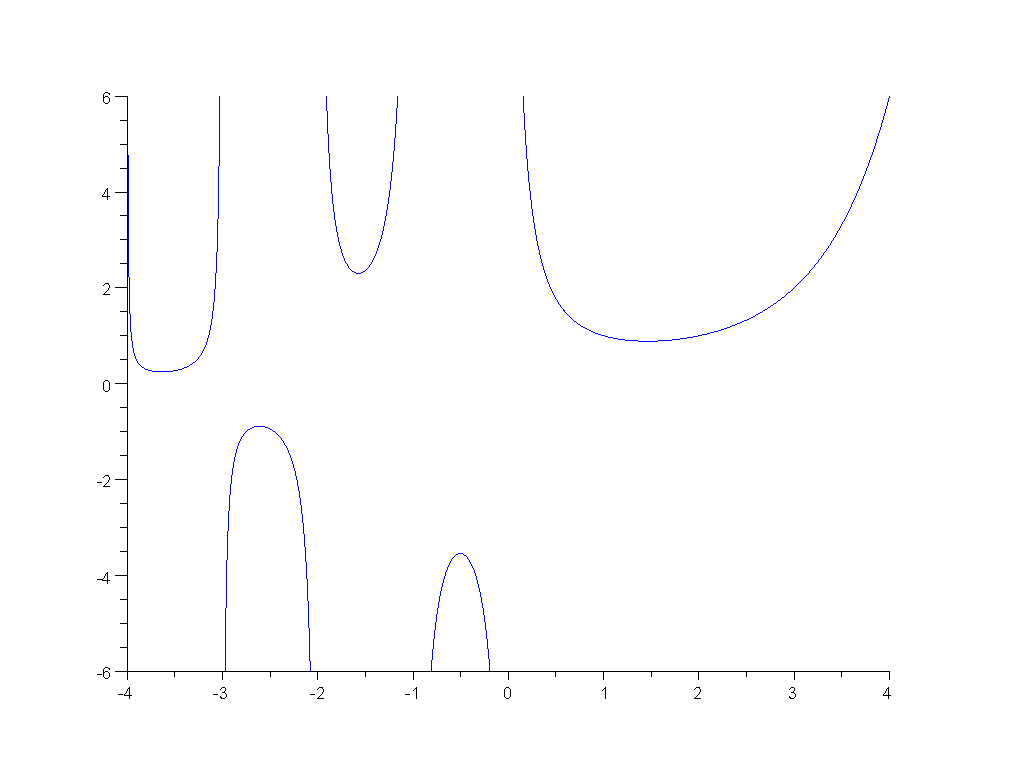
\includegraphics[width=10cm]{introdiscreteprobas/gamma_function.pdf}
\end{center}
\caption{The gamma function.}
\label{fig-introstats-gamma}
\end{figure}

The following session presents various values of the \scifun{gamma}
function.
\lstset{language=scilabscript}
\begin{lstlisting}
-->x = [-2 -1 -0 +0 1 2 3 4 5 6]';
-->[x gamma(x)]
 ans  =
  - 2.   Nan    
  - 1.   Nan    
    0.  -Inf    
    0.   Inf    
    1.    1.    
    2.    1.    
    3.    2.    
    4.    6.    
    5.    24.   
    6.    120.  
\end{lstlisting}

Notice that the two floating point signed zeros \scivar{+0} and \scivar{-0} are associated 
with the function values $-\infty$ and $+\infty$. This is consistent 
with the value of the limit of the function from either sides 
of the singular point. 
This contrasts with the value of the gamma function on negative 
integer points, where the function value is \scivar{\%nan}.
This is consistent with the fact that, on this singular points, 
the function is equal to $-\infty$ on one side and $+\infty$ on the other side.
Therefore, since the argument $x$ has one single floating 
point representation when it is a negative nonzero integer, the only 
solution consistent with the IEEE754 standard is to set the result to \scivar{\%nan}.

Notice that we used 1001 points to plot the gamma function. This 
allows to get points exactly located at the singular points.
These values are ignored by the \scifun{plot} function and 
makes a nice plot. Indeed, if 1000 points are used instead, vertical
lines corresponding to the y-value immediately at the left and 
the right of the singularity would be displayed.

%%%%%%%%%%%%%%%%%%%%%%%%%%%%%%%%%%%%%%%%%%%%%%%%%%%%%%%%%%%%%%%%%%%%%%%%%%%%%%%%%%%%%%%

\subsection{The factorial and log-factorial functions}

In the following script, we plot the \scifun{factorial} function  
for values of $n$ from 1 to 10.
\lstset{language=scilabscript}
\begin{lstlisting}
f = factorial(1:10)
plot ( 1:10 , f , "b-o" )
\end{lstlisting}
The result is presented in figure \ref{fig-introstats-fact}.
We see that the growth rate of the factorial function is large.

\begin{figure}
\begin{center}
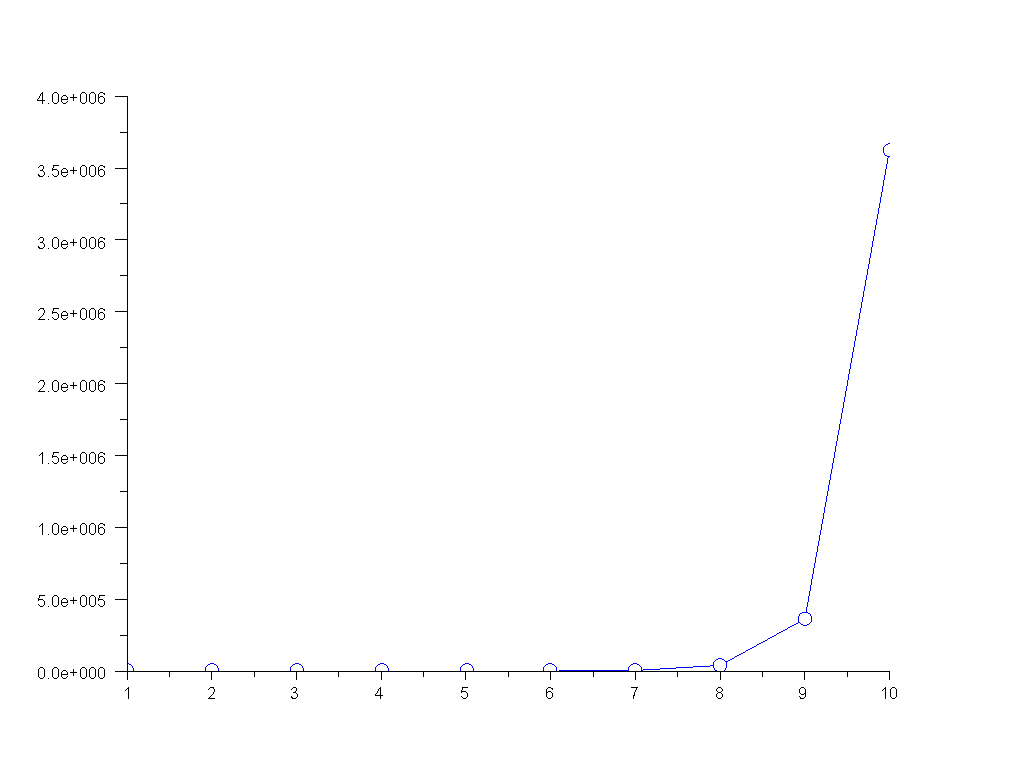
\includegraphics[width=10cm]{introdiscreteprobas/factorial.pdf}
\end{center}
\caption{The factorial function.}
\label{fig-introstats-fact}
\end{figure}

The largest values of $n$ so that $n!$ is representable as a 
double precision floating point number is $n=170$.
In the following session, we check that $171!$ is not representable 
as a Scilab double.
\lstset{language=scilabscript}
\begin{lstlisting}
-->factorial(170)
 ans  =
    7.257+306  
-->factorial(171)
 ans  =
   Inf  
\end{lstlisting}

The factorial function is implied in many probability computations,
sometimes as an intermediate result. Since it grows so fast, we might 
be interested in computing its order of magnitude instead of its value.
Let us introduce the function $f_{ln}$ as the logarithm of the factorial 
number $n!$:
\begin{eqnarray}
\label{exercise-hypergeometric5}
f_{ln}(n) = \ln (n!).
\end{eqnarray}
Notice that we used the base-$e$ logarithm function $\ln$, that is, the 
reciprocal of the exponential function. 

The factorial number $n!$ grows exponentially, 
but its logarithm grows much more slowly. In the figure \ref{fig-introstats-logfact}, 
we plot the logarithm of $n!$ in the interval $[0,170]$. 
We see that the y coordinate varies only from 0 up to 800.
Hence, there are a large number of integers $n$ for which $n!$ may be not 
representable as a double but $f_{ln}(n)$ is still representable as a double.

\begin{figure}
\begin{center}
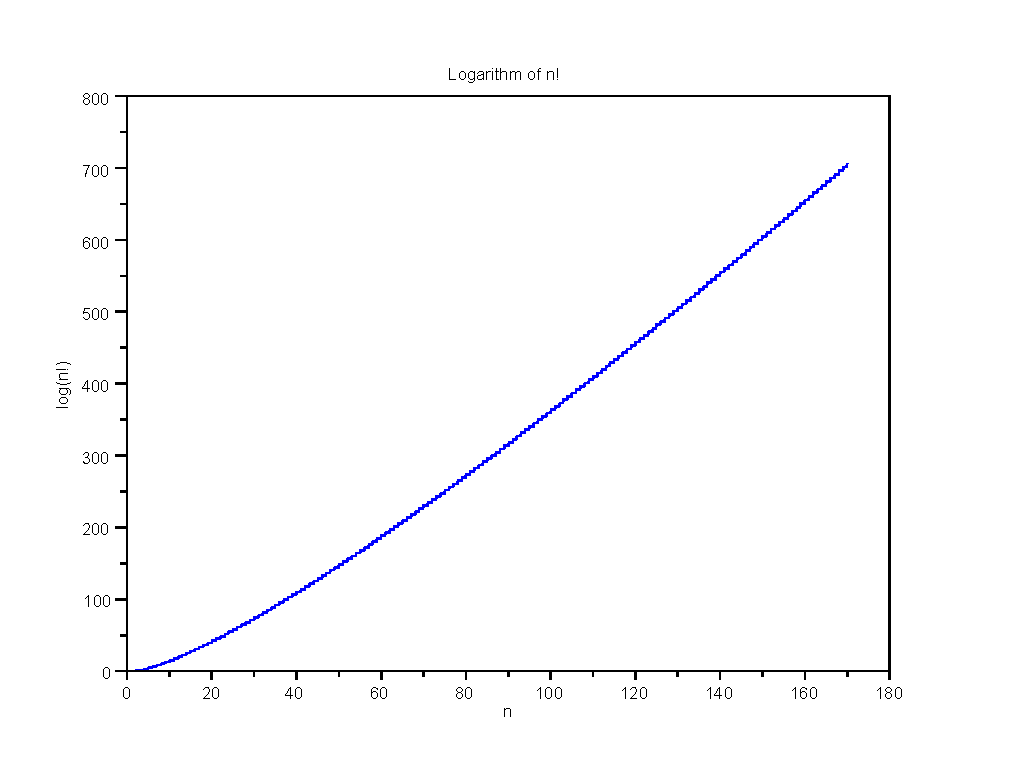
\includegraphics[width=10cm]{introdiscreteprobas/log_factorial.pdf}
\end{center}
\caption{Logarithm of the factorial number.}
\label{fig-introstats-logfact}
\end{figure}

%%%%%%%%%%%%%%%%%%%%%%%%%%%%%%%%%%%%%%%%%%%%%%%%%%%%%%%%%%%%%%%%%%%%%%%%%%%%%%%%%%%%%%%
\subsection{Computing factorial and log-factorial with Scilab}

In this section, we present how to compute the factorial function in Scilab. 
We focus in this section on accuracy and efficiency.

\index{factorial}
The \scifun{factorial} function returns the factorial 
number associated with the given $n$. It has the following 
syntax:
\lstset{language=scilabscript}
\begin{lstlisting}
f = factorial ( n )
\end{lstlisting}
In the following session, we compute $n!$ for 
several values of $n$, from 1 to 7.
\lstset{language=scilabscript}
\begin{lstlisting}
-->n = (0:7)';
-->[n factorial(n)]
 ans  =
    0.    1.     
    1.    1.     
    2.    2.     
    3.    6.     
    4.    24.    
    5.    120.   
    6.    720.   
    7.    5040.  
\end{lstlisting}

The implementation of the \scifun{factorial} function in Scilab
allows to take both matrix and hypermatrices input arguments.
In order to be fast, it uses vectorization. 
The following \scifun{factorialScilab} function represents the 
computationnal core of the actual implementation of 
the \scifun{factorial} function in Scilab.
\lstset{language=scilabscript}
\begin{lstlisting}
function f = factorialScilab ( n )
  n(n==0)=1
  t = cumprod(1:max(n))
  v = t(n(:))
  f = matrix(v,size(n))
endfunction
\end{lstlisting}
The statement \scivar{n(n==0)=1} allows to set all zeros of 
the matrix \scivar{n} to one, so that the next statements 
do not have to manage the special case $0!=1$.
Then, we use the \scifun{cumprod} function in order to compute 
a column vector containing cumulated products, up to the maximum entry of \scivar{n}.
The use of \scifun{cumprod} allows to get all the results 
in one call, but also produces unnecessary values of the factorial 
function. In order to get just what is needed, the statement 
\scivar{v = t(n(:))} allows to extract the required values.
Finally, the statement \scivar{f = matrix(v,size(n))} reshapes the 
matrix of values so that the shape of the output argument is the 
same as the shape of the input argument.

The following function allows to compute $n!$ based on the
\scifun{prod} function, which computes the product of its 
input argument.
\lstset{language=scilabscript}
\begin{lstlisting}
function f = factorial_naive ( n )
  f = prod(1:n)
endfunction
\end{lstlisting}
The \scifun{factorial\_naive} function has two drawbacks. 
The first one is that it cannot manage matrix input 
arguments. Furthermore, it requires more memory than necessary.

In practice, the factorial function can be computed based on the 
gamma function. The following implementation of the factorial 
function is based on the equality \ref{prop-gammafact2}.
\lstset{language=scilabscript}
\begin{lstlisting}
function f = myfactorial ( n )
  if ( ( or (n(:) <  0) ) | ( n(:) <> round (n(:) ) ) ) then
    error ("myfactorial: n must all be nonnegative integers");
  end
  f = gamma ( n + 1 )
endfunction
\end{lstlisting}
The \scifun{myfactorial} function also checks that the input argument 
\scivar{n} is positive. It also checks that \scivar{n} is an integer by 
using the condition \scivar{( n(:) <> round (n(:) )}.
Indeed, if the value of \scivar{n} is different from the value of \scivar{round(n)},
this means that the input argument \scivar{n} is not an integer. 

The main drawback of the \scifun{factorialScilab} function 
is that it uses more memory than necessary. It may fail to produce 
a result when it is given a large input argument.
In the following session, we use the \scifun{factorial} function
with a very large input integer. 
In this particular case, it is obvious that the correct result 
is \scivar{Inf}. Anyway, this should have been the result 
of the function, which should not have generated an error.
On the other side, the \scifun{myfactorial} function works 
perfectly.
\lstset{language=scilabscript}
\begin{lstlisting}
-->factorial(1.e10)
 !--error 17 
stack size exceeded!
-->myfactorial(1.e10)
 ans  =
   Inf  
\end{lstlisting}

We now consider the computation of the log-factorial function $f_{ln}$.
We can use the \scifun{gammaln} function which directly provides the 
correct result.
\lstset{language=scilabscript}
\begin{lstlisting}
function flog = factoriallog ( n )
  flog = gammaln(n+1);
endfunction
\end{lstlisting}
The advantage of this method is that matrix input arguments 
can be manage by the \scifun{factoriallog} function.

%%%%%%%%%%%%%%%%%%%%%%%%%%%%%%%%%%%%%%%%%%%%%%%%%%%%%%%%%%%%%%%%%%%%%%%%%%%%%%%%%%%%%%%
\subsection{Computing permutations and log-permutations with Scilab}
\label{sec-computeperm}

\index{permutations}
There is no Scilab function to compute the number of 
permutations $(n)_j = n.(n-1)\ldots (n-j+1)$.

We might be interested in simplifying the 
expression for the permutation number
We have 
\begin{eqnarray}
(n)_j &=& n . (n-1) \ldots (n-j+1) \\
&=& \frac{n . (n-1) . \ldots . 1}{(n-j).(n-j-1)\ldots 1},\\
&=&\frac{n!}{(n-j)!}. \label{sec-computeperm1}
\end{eqnarray}
This leads to the following function \scifun{permutations\_verynaive}.
\lstset{language=scilabscript}
\begin{lstlisting}
function p = permutations_verynaive ( n , j )
  p = factorial(n)./factorial(n-j)
endfunction
\end{lstlisting}
In the following session, we see that the previous function 
works for small values of $n$ and $j$.
\lstset{language=scilabscript}
\begin{lstlisting}
-->n = [5 5 5 5 5 5]';
-->j = [0 1 2 3 4 5]';
-->[n j permutations_verynaive(n,j)]
 ans  =
    5.    0.    1.    
    5.    1.    5.    
    5.    2.    20.   
    5.    3.    60.   
    5.    4.    120.  
    5.    5.    120.  
\end{lstlisting}
In the following session, we compute the permutations number 
$(171)_{171} = 171!$. 
\lstset{language=scilabscript}
\begin{lstlisting}
-->permutations_verynaive ( 171 , 171 )
 ans  =
   Inf  
\end{lstlisting}
This is caused by an overflow during the computation of 
the factorial function. There is unfortunately no way 
to fix this problem, since the result is, indeed, not 
representable as a double precision floating point number.

On the other hand, the \scifun{permutations\_verynaive} function 
performs poorly in cases where $n$ is large, whatever the value of 
$j$, as presented in the following session.
\lstset{language=scilabscript}
\begin{lstlisting}
-->permutations_verynaive ( 171 , 0 )
 ans  =
   Nan  
\end{lstlisting}
There is certainly something to do about this problem, since,
when $j=0$, we have $(n)_0=1$. 

The following \scifun{permutations\_naive} function allows to compute $(n)_j$ for 
positive integer values of $n,j$.
It is based on the \scifun{prod} function, which computes the 
product of the given vector.
\lstset{language=scilabscript}
\begin{lstlisting}
function p = permutations_naive ( n , j )
  p = prod ( n-j+1 : n )
endfunction
\end{lstlisting}
In the following session, we check the values of the 
function $(n)_j$ for $n=5$ and $j=1,2,\ldots,5$.
\lstset{language=scilabscript}
\begin{lstlisting}
-->n = 5;
-->for j = 0 : 5
-->  p = permutations_naive ( n , j );
-->  disp([n j p]);
-->end
    5.    0.    1.  
    5.    1.    5.  
    5.    2.    20.  
    5.    3.    60.  
    5.    4.    120.  
    5.    5.    120.  
\end{lstlisting}

The following session shows that \scifun{permutations\_naive} 
performs more nicely than the previous function for small 
values of $j$.
\lstset{language=scilabscript}
\begin{lstlisting}
-->permutations_naive ( 171 , 0 )
 ans  =
    1.  
\end{lstlisting}

The \scifun{permutations\_naive} function has still several drawbacks.
First, it requires more memory than necessary. 
For example, it may fail to compute $(n)_n=1$ for values of 
$n$ larger than $10^5$. 
\lstset{language=scilabscript}
\begin{lstlisting}
-->permutations_naive ( 1.e7 , 1.e7 )
 !--error 17 
stack size exceeded!
\end{lstlisting}

Furthermore, the function \scifun{permutations\_naive} does not manage 
matrix input arguments. 

In order to accurately compute the permutation number, we may compute its 
logarithm first. 
By the equation \ref{sec-computeperm1}, we have 
\begin{eqnarray}
\ln((n)_j) 
&=& \ln\left(\frac{n!}{(n-j)!}\right) \\
&=& \ln(n!) - \ln((n-j)!) \\
&=& \ln(\Gamma(n+1)) - \ln(\Gamma(n-j+1)).
\end{eqnarray}
The previous equation leads to the definition of the log-permutation 
function, as defined in the following function.
\lstset{language=scilabscript}
\begin{lstlisting}
function plog = permutationslog ( n , j )
  plog = gammaln(n+1)-gammaln(n-j+1);
endfunction
\end{lstlisting}
In order to compute the permutation number, we compute the exponential of the 
expression. This leads to the following function \scifun{permutations},
where we round the result in order to get integer results.
\lstset{language=scilabscript}
\begin{lstlisting}
function p = permutations ( n , j )
  p = exp(gammaln(n+1)-gammaln(n-j+1));
  if ( and(round(n)==n) & and(round(j)==j) ) then
    p = round ( p )
  end
endfunction
\end{lstlisting}

The \scifun{permutations} function takes matrix input arguments, as presented in the 
following session. 
\lstset{language=scilabscript}
\begin{lstlisting}
-->n = [5 5 5 5 5 5]';
-->j = [0 1 2 3 4 5]';
-->[n j permutations(n,j)]
 ans  =
    5.    0.    1.    
    5.    1.    5.    
    5.    2.    20.   
    5.    3.    60.   
    5.    4.    120.  
    5.    5.    120.  
\end{lstlisting}

Finally, the \scifun{permutations} functions requires the minimum amount of memory
and performs correctly, even for large values of $n$.
\lstset{language=scilabscript}
\begin{lstlisting}
-->permutations ( 1.e7 , 1.e7 )
 ans  =
   Inf  
-->permutations ( 1.e7 , 0 )
 ans  =
    1.  
\end{lstlisting}

%%%%%%%%%%%%%%%%%%%%%%%%%%%%%%%%%%%%%%%%%%%%%%%%%%%%%%%%%%%%%%%%%%%%%%%%%%%%%%%%%%%%%%%
\subsection{Combinations}
\label{section-combinaison}

\index{combination}
In this section, we present combinations, which are unordered subsets
of a given set.

The number of distinct subsets with $j$ elements which can be chosen from
a set $A$ with $n$ elements is the binomial coefficient and is denoted by 
$\choosefun{n}{j}$. The following proposition gives an explicit formula 
for the binomial number.

\index{binomial}
\begin{proposition}
(\emph{Binomial})
The number of distinct subsets with $j$ elements which can be chosen from
a set $A$ with $n$ elements is the binomial coefficient and is defined by 
\begin{eqnarray}
\label{introstats-eq-binomial}
\choosefun{n}{j} = \frac{n . (n-1) \ldots (n-j+1)}{1.2 \ldots j}.
\end{eqnarray}
\end{proposition}

The following proof is based on the fact that subsets are unordered, while 
permutations are based on the order.

\begin{proof}
Assume that the set $A$ has $n$ elements and consider subsets with $j>0$ elements.
By proposition \ref{propo-permutation}, the number of $j$-permutations of the set $A$ is 
$(n)_j = n . (n-1) \ldots (n-j+1)$.
Notice that the order does not matter in creating the subsets, so that the number 
of subsets is lower than the number of permutations.
This is why each subset is associated with one or more permutations.
By proposition \ref{propo-factorial}, there are $j!$ ways to order a 
set with $j$ elements. Therefore, the number of subsets with $j$ elements
is given by $\choosefun{n}{j} = \frac{n . (n-1) . \ldots . (n-j+1)}{1.2 \ldots j}$, 
which concludes the proof.
\end{proof}

The expression for the binomial coefficient can be simplified if we 
use the number of $j$-permutations and the factorial number, which leads 
to 
\begin{eqnarray}
\choosefun{n}{j} = \frac{(n)_j}{j!}.
\end{eqnarray}
The equality $(n)_j = \frac{n!}{(n-j)!}$ leads to 
\begin{eqnarray}
\choosefun{n}{j} = \frac{n!}{(n-j)!j!}. \label{section-combinaison1}
\end{eqnarray}
This immediately leads to 
\begin{eqnarray}
\choosefun{n}{j} = \choosefun{n}{n-j}.
\end{eqnarray}

The following proposition shows a recurrence relation for 
binomial coefficients.

\begin{proposition}
\label{introstats-recurrencebinomial}
For integers $n>0$ and $0<j<n$, the binomial coefficients satisfy
\begin{eqnarray}
\choosefun{n}{j} = \choosefun{n-1}{j} + \choosefun{n-1}{j-1}.
\end{eqnarray}
\end{proposition}

The proof recurrence relation of the proposition \ref{introstats-recurrencebinomial}
is given as an exercise.

%%%%%%%%%%%%%%%%%%%%%%%%%%%%%%%%%%%%%%%%%%%%%%%%%%%%%%%%%%%%%%%%%%%%%%%%%%%%%%%%%%%%%%%
\subsection{Computing combinations with Scilab}
\label{introstats-computingcombinations}
In this section, we show how to compute combinations with 
Scilab. 

There is no Scilab function to compute the binomial number 
$\choosefun{n}{j}$. 
In order to compute the required combinations, we will use 
the gamma function. By the equation \ref{section-combinaison1}, 
we have
\begin{eqnarray}
\ln\left( \choosefun{n}{j} \right)
&=& \ln(n!)- \ln((n-j)!) - \ln(j!) \\
&=& \ln(\Gamma(n+1))- \ln(\Gamma(n-j+1)) - \ln(\Gamma(j+1)).
\end{eqnarray}
The following Scilab function performs 
the computation of the binomial number for positive values of $n$ and $j$.
\lstset{language=scilabscript}
\begin{lstlisting}
function c = combinations ( n , j )
  c = exp(gammaln(n+1)-gammaln(j+1)-gammaln(n-j+1));
  if ( and(round(n)==n) & and(round(j)==j) ) then
    b = round ( b )
  end
endfunction
\end{lstlisting}

In the following session, we compute the value of the binomial 
coefficients for $n=1,2,\ldots,5$. The values in this table 
are known as Pascal's triangle.
\lstset{language=scilabscript}
\begin{lstlisting}
-->for n=0:5
-->  for j=0:n
-->    c = combinations ( n , j );
-->    mprintf("%2d   ",c);
-->  end
-->  mprintf("\n");
-->end
 1   
 1    1   
 1    2    1   
 1    3    3    1   
 1    4    6    4    1   
 1    5   10   10    5    1   
\end{lstlisting}

We now explain why we choose to use the \scifun{exp} and the 
\scifun{gammaln} to perform our computation for the \scifun{combinations}
function. Indeed, we could have used a more naive method, based on the 
\scifun{prod} function, as in the following example :
\lstset{language=scilabscript}
\begin{lstlisting}
function c = combinations_naive ( n , j )
  c = prod ( n : -1 : n-j+1 )/prod(1:j)
endfunction
\end{lstlisting}

For small integer values of $n$, the two previous functions 
produce the same result. Unfortunately, even for moderate 
values of $n$, the naive method fails. In the following session, we 
compute the value of $\choosefun{n}{j}$ with $n=10000$ and 
$j=134$.
\lstset{language=scilabscript}
\begin{lstlisting}
-->combinations ( 10000 , 134 )
 ans  =
    2.050+307  
-->combinations_naive ( 10000 , 134 )
 ans  =
   Inf  
\end{lstlisting}

The reason why the naive computation fails is because the products 
involved in the intermediate variables for the naive method are 
generating an overflow. This means that the values are too large 
for being stored in a double precision floating point variable.
This is a pity, since the result can be stored in a double precision
floating point variable. The \scifun{combinations} function, on the 
other hand, computes first the logarithm of the factorial number. This 
logarithm cannot overflow because if \scivar{x} is a double precision 
floating point number, then \scivar{log(x)} can always be 
represented since its exponent is always smaller than the exponent 
of \scivar{x}. In the end, the combination of the \scivar{exp}
and \scivar{gammaln} functions allows to accurately compute the 
result in the sense that, if the result is representable as 
a double precision floating point number, then \scifun{combinations}
will produce a result as accurate as possible.

Notice that we use the \scifun{round} function in our implementation of 
the \scifun{combinations} function. This is because the \scifun{combinations}
function manages in fact real double precision floating point input arguments. 
Consider the example where $n=4$ and $j=1$ and let us compute the 
associated number of combinations $\choosefun{n}{j}$.
In the following Scilab session, we use the \scifun{format} so that we display
at least 15 significant digits.
\lstset{language=scilabscript}
\begin{lstlisting}
-->format(20);
-->n = 4;
-->j = 1;
-->c = exp(gammaln(n+1)-gammaln(j+1)-gammaln(n-j+1))
 c  =
    3.99999999999999822  
\end{lstlisting}
We see that there are 15 significant digits, which is the best 
that can be expected from the \scifun{exp} and \scifun{gammaln}
functions. But the result is not an integer anymore, i.e. it is very
close to the integer 4, but not exactly equal to it. 
This is why in the \scifun{combinations} function, if $n$ and $j$ 
are both integers, we round the number $c$ to the nearest integer
with a call to the \scifun{round} function.

Finally, notice that our implementation of the \scifun{combinations} 
function uses the function \scifun{and}. This allows to use 
arrays of integers as input variables. In the following 
session, we compute $\choosefun{5}{j}$, for $j=0,1,\ldots,5$ 
in one single call. This is a consequence of the fact that the \scifun{exp} 
and \scifun{gammaln} both accept matrices input arguments.
\lstset{language=scilabscript}
\begin{lstlisting}
-->n = 5 * ones(6,1);
-->j = (0:5)';
-->c = combinations ( n , j );
-->[n j c]
 ans  =
    5.    0.    1.   
    5.    1.    5.   
    5.    2.    10.  
    5.    3.    10.  
    5.    4.    5.   
    5.    5.    1.   
\end{lstlisting}

%%%%%%%%%%%%%%%%%%%%%%%%%%%%%%%%%%%%%%%%%%%%%%%%%%%%%%%%%%%%%%%%%%%%%%%%%%%%%%%%%%%%%%%
\subsection{The poker game}
In the following example, we use Scilab to compute the probabilities 
of poker hands.

\index{poker}
\index{rank}
\index{suit}

The poker game is based on a 52 cards deck, which is presented in
figure \ref{fig-introstats-52cards}. Each card can have one of the 13 available \emph{ranks}
from $1$ to $K$, and have on the 4 available \emph{suits} $\Box$, $\heartsuit$, $\clubsuit$ and $\spadesuit$.
Each player receives 5 cards randomly chosen in the deck. Each player tries to combine the cards to 
form a well-known combination of cards as presented in the figure \ref{fig-introstats-winpoker}.
Depending on the combination, the player can beat, or be defeated by another player. 
The winning combination is the rarest; that is, the one which has the 
lowest probability. In figure \ref{fig-introstats-winpoker}, the combinations 
are presented in decreasing order of probability.

\begin{figure}
\begin{center}
\begin{tabular}{|l|}
\hline
1$\Box$ 2$\Box$ 3$\Box$ 4$\Box$ 5$\Box$ 6$\Box$ 7$\Box$ 8$\Box$ 9$\Box$ 10$\Box$ J$\Box$ Q$\Box$ K$\Box$\\
1$\heartsuit$ 2$\heartsuit$ 3$\heartsuit$ 4$\heartsuit$ 5$\heartsuit$ 6$\heartsuit$ 7$\heartsuit$ 8$\heartsuit$ 9$\heartsuit$ 10$\heartsuit$ J$\heartsuit$ Q$\heartsuit$ K$\heartsuit$\\
1$\clubsuit$ 2$\clubsuit$ 3$\clubsuit$ 4$\clubsuit$ 5$\clubsuit$ 6$\clubsuit$ 7$\clubsuit$ 8$\clubsuit$ 9$\clubsuit$ 10$\clubsuit$ J$\clubsuit$ Q$\clubsuit$ K$\clubsuit$\\
1$\spadesuit$ 2$\spadesuit$ 3$\spadesuit$ 4$\spadesuit$ 5$\spadesuit$ 6$\spadesuit$ 7$\spadesuit$ 8$\spadesuit$ 9$\spadesuit$ 10$\spadesuit$ J$\spadesuit$ Q$\spadesuit$ K$\spadesuit$\\
\hline
\end{tabular}
\end{center}
\caption{Cards of a 52 cards deck - "J" stands for Jack, "Q" stands for Queen and "K" stands for King}
\label{fig-introstats-52cards}
\end{figure}

\begin{figure}
\begin{center}
\begin{tabular}{|lll|}
\hline
Name & Description & Example \\
\hline
no pair & none of the below combinations & 7$\Box$ 3$\clubsuit$ 6$\clubsuit$ 3$\heartsuit$ 1$\spadesuit$\\
pair & two cards of the same rank & Q$\clubsuit$ Q$\clubsuit$ 2$\heartsuit$ 3$\clubsuit$ 1$\Box$\\
double pair & 2$\times$ two cards of the same rank & 2$\Box$ 2$\spadesuit$ Q$\spadesuit$ Q$\clubsuit$\\
three of a kind & three cards of the same rank & 2$\Box$ 2$\spadesuit$ 2$\heartsuit$ 3$\clubsuit$ 1$\Box$\\
straight & five cards in a sequence, not all the same suit & 3$\heartsuit$ 4$\spadesuit$ 5$\Box$ 6$\spadesuit$ 7$\Box$\\
flush & five cards in a single suit & 2$\Box$ 3$\Box$ 7$\Box$ J$\Box$ K$\Box$\\
full house & one pair and one triple, each of the same rank & 2$\Box$ 2$\spadesuit$ 2$\heartsuit$ Q$\clubsuit$ Q$\heartsuit$\\
four of a kind & four cards of the same rank & 5$\Box$ 5$\spadesuit$ 5$\clubsuit$ 5$\heartsuit$ 2$\heartsuit$\\
straight flush & five in a sequence in a single suit& 2$\Box$ 3$\Box$ 4$\Box$ 5$\Box$ 6$\Box$\\
royal flush & 10, J, Q, K, 1 in a single suit & 10$\spadesuit$ J$\spadesuit$ Q$\spadesuit$ K$\spadesuit$ 1$\spadesuit$ \\
\hline
\end{tabular}
\end{center}
\caption{Winning combinations at the Poker}
\label{fig-introstats-winpoker}
\end{figure}

Even if winning at this game requires some understanding of human 
psychology, understanding probabilities can help. 
Why does the \emph{four of a kind} beats the \emph{full house} ?

To answer this question, we will compute the probability of each event.
Since the order of the cards can be changed by the player, we are interested 
in combinations (and not in permutations).
We make the assumption that the process of choosing the cards is really random,
so that all combinations of 5 cards have the same probabilities, i.e.
the distribution function is uniform.
Since the order of the cards does not matter, the sample space $\Omega$ 
is the set of all combinations of 5 cards chosen from 52 cards. Therefore, 
the size of $\Omega$ is
\begin{eqnarray}
\#{\Omega} = \choosefun{52}{5} = 2598960.
\end{eqnarray}

The probability of a \emph{four of a kind} is computed as follows.
In a 52-cards deck, there are 13 different \emph{four of a kind} combinations.
Since the 5-th card is chosen at random from the 48 remaining cards, there 
are $13.48$ different \emph{four of a kind}. The probability of a \emph{four of a kind} is 
therefore 
\begin{eqnarray}
P(\textrm{four of a kind}) = \frac{13.48}{\choosefun{52}{5}.} 
= \frac{624}{2598960} \approx 0.0002401
\end{eqnarray}

The probability of a \emph{full house} is computed as follows.
There are 13 different ranks in the deck, and, once a rank is chosen, there
are $\choosefun{4}{2}$ different pairs for one rank Therefore the total number 
of pairs is $13.\choosefun{4}{2}$. Once the pair is set, there are 
12 different ranks to choose for the triple and there are $\choosefun{4}{3}$
different triples for one rank. The total number of \emph{full house} is 
therefore $13.\choosefun{4}{2}.12.\choosefun{4}{3}$. Notice that the 
triple can be chosen first, and the pair second, but this would lead
exactly to the same result. Therefore, the probability of a \emph{full house} is
\begin{eqnarray}
P(\textrm{full house}) 
= \frac{13.12.\choosefun{4}{2}.\choosefun{4}{3}}{\choosefun{52}{5}.} 
= \frac{3744}{2598960}
\approx 0.0014406
\end{eqnarray}

The computation of all the probabilities of the winning combinations 
is given as exercise.

%%%%%%%%%%%%%%%%%%%%%%%%%%%%%%%%%%%%%%%%%%%%%%%%%%%%%%%%%%%%%%%%%%%%%%%%%%%%%%%%%%%%%%%
\subsection{Bernoulli trials}

In this section, we present Bernoulli trials and the binomial discrete 
distribution function. We give the example of a coin tossed several times as an example 
of such a process.

\index{Bernoulli}
\begin{definition}
A Bernoulli trials process is a sequence of $n>0$ experiments 
with the following rules.
\begin{enumerate}
\item Each experiment has two possible outcomes, which we may call
success and failure.
\item The probability $p\in[0,1]$ of success of each experiment is the same for each
experiment. 
\end{enumerate}
\end{definition}

In a Bernoulli process, the probability $p$ of success is not changed by any knowledge of previous 
outcomes
For each experiment, the probability $q$ of failure is $q=1-p$.

It is possible to represent a Bernoulli process with a tree diagram, as 
the one in figure \ref{fig-introstats-bernouillitree}.

\begin{figure}
\begin{center}
\includegraphics[width=7cm]{introdiscreteprobas/tree-Bernoulli.pdf}
\end{center}
\caption{A Bernoulli process with 3 trials. -- The letter "S" indicates "success" and the letter 
"F" indicates "failure".}
\label{fig-introstats-bernouillitree}
\end{figure}

A complete experiment is a sequence of success and failures, which can 
be represented by a sequence of S's and F's.
Therefore the size of the sample space is $\#(\Omega)=2^n$, which 
is equal to $2^3=8$ in our particular case of 3 trials.

By definition, the result of each trial is independent from the result of 
the previous trials. Therefore, the 
probability of an event is the product of the probabilities of each 
outcome. 

Consider the outcome $x="SFS"$ for example. The value of the 
distribution function $f$ for this outcome is
\begin{eqnarray}
f(x="SFS") = pqp = p^2q.
\end{eqnarray}
The table \ref{fig-introstats-probabernouilli} presents the value of the distribution function
for each outcome $x\in \Omega$.

\begin{figure}
\begin{center}
\begin{tabular}{|ll|}
\hline
$x$ & $f(x)$\\
\hline
SSS & $p^3$\\
SSF & $p^2 q$\\
SFS & $p^2 q$\\
SFF & $p q^2$\\
FSS & $p^2 q$\\
FSF & $p q^2$\\
FFS & $p q^2$\\
FFF & $q^3$\\
\hline
\end{tabular}
\end{center}
\caption{Probabilities of a Bernoulli process with 3 trials}
\label{fig-introstats-probabernouilli}
\end{figure}

We can check that the sum of probabilities of all events is equal to 1.
Indeed, 
\begin{eqnarray}
\sum_{i=1,8} f(x_i)&=& p^3 + p^2 q + p^2 q + p q^2 + p^2 q + p q^2 + p q^2 + q^3\\
&=& p^3 + 3 p^2 q + 3 p q^2 + q^3\\
&=& ( p + q )^3\\
&=& 1
\end{eqnarray}

We denote by $b(n,p,j)$ the probability that, in $n$ Bernoulli trials with 
success probability $p$, there are exactly $j$ successes. 
In the particular case where there are $n=3$ trials, the figures \ref{fig-introstats-bernouillitree}
and \ref{fig-introstats-probabernouilli}
gives the following results:
\begin{eqnarray}
b(3,p,3) &=& p^3\\
b(3,p,2) &=& 3 p^2 p\\
b(3,p,1) &=& 3 p q^2\\
b(3,p,0) &=& q^3
\end{eqnarray}

The following proposition extends the previous analysis to the 
general case.

\begin{proposition}
(\emph{Binomial probability})
\label{introstats-prop-binomialdist}
In a Bernoulli process with $n>0$ trials with success probability $p\in[0,1]$, the probability
of exactly $j$ successes is 
\begin{eqnarray}
b(n,p,j) = \choosefun{n}{j} p^j q^{n-j},
\end{eqnarray}
where $0\leq j \leq n$ and $q=1-p$.
\end{proposition}

\begin{proof}
We denote by $A\subset \Omega$ the event that one process is associated with exactly $j$ successes. 
By definition, the probability of the event $A$ is 
\begin{eqnarray}
b(n,p,j) = P(A) = \sum_{x\in A} f(x).
\end{eqnarray}
Assume that an outcome $x\in \Omega$ is associated with exactly $j$ successes. Since there are 
$n$ trials, the number of failures is $n-j$. That means that the value of the distribution
function of this outcome $x\in A$ is $f(x) = p^j q^{n-j}$.
Since all the outcomes $x$ in the set $A$ have the same distribution function value, 
we have
\begin{eqnarray}
\label{introstats-eq-bnpj}
b(n,p,j) = \#(A) p^j q^{n-j}.
\end{eqnarray}
The size of the set $A$ is the number of subsets of $j$ elements in a set of size $n$.
Indeed, the order does not matter since we only require that, during the whole 
process, the total number of successes is exactly $j$, no matter of the order 
of the successes and failures.
The number of outcomes with exactly $j$ successes is therefore $\#(A)=\choosefun{n}{j}$,
which, combined with equation \ref{introstats-eq-bnpj}, concludes the proof. 
\end{proof}

\begin{example}
A fair coin is tossed six times. What is the probability that 
exactly 3 heads turn up~? This process is a Bernoulli process
with $n=6$ trials. Since the coin is fair, the probability 
of success at each trial is $p=1/2$. We can apply proposition \ref{introstats-prop-binomialdist}
with $j=3$ and get 
\begin{eqnarray}
b(6,1/2,3) = \choosefun{6}{3} (1/2)^3 (1/2)^3 \approx 0.3125,
\end{eqnarray}
so that the probability of having exactly 3 heads is 0.3125.
\end{example}

%%%%%%%%%%%%%%%%%%%%%%%%%%%%%%%%%%%%%%%%%%%%%%%%%%%%%%%%%%%%%%%%%%%%%%%%%%%%%%%%%%%%%%%

\section{Simulation of random processes with Scilab}
\label{introstats-simulation}

In this section, we present how to simulate random 
events with Scilab. The problem of generating 
random numbers is more complex and will not be detailed 
in this chapter. 
We begin by a brief overview of random number 
generation and detail the random number generator used in
the \scifun{rand} function. Then we analyze how to generate 
random numbers in the interval $[0,1]$ with the \scifun{rand} function. We 
present how to generate random integers in a given interval $[0,m-1]$ or $[m_1,m_2]$.
In the final part, we present a practical simulation of 
a game based on tossing a coin.

%%%%%%%%%%%%%%%%%%%%%%%%%%%%%%%%%%%%%%%%%%%%%%%%%%%%%%%%%%%%%%%%%%%%%%%%%%%%%%%%%%%%%%%
\subsection{Overview}

In this section, we present a special class of random
number generators so that we can have a general
representation of what exactly this means.

The goal of a uniform random number generator is to generate
a sequence of real values $u_n\in [0,1]$ for $n\geq 0$.
Most uniform random number generators are based on the 
fraction 
\begin{eqnarray}
u_n = \frac{x_n}{m}
\end{eqnarray}
where $m$ is a large 
integer and $x_n$ is a positive integer so that $0<x_n<m$ .
In many random number generators, the integer $x_{n+1}$ is 
computed from the previous element in the sequence $x_n$.

The linear congruential generators 
\cite{artcomputerKnuthVol2} are based on the sequence
\begin{eqnarray}
x_{n+1} = (a x_n + c) \pmod{m},
\end{eqnarray}
where 
\begin{itemize}
\item $m$ is the modulus satisfying $m>0$,
\item $a$ is the multiplier satisfying $0\leq a <m$,
\item $c$ is the increment satisfying $0\leq c <m$,
\item $x_0$ is the starting value satisfying $0\leq x_0 <m$.
\end{itemize}

The parameters $m$, $a$, $c$ and $x_0$ should satisfy
several conditions so that the sequence $x_n$ has 
good statistical properties. 
Indeed, naive approaches leads to poor results in this matter.
For example, consider the example where $x_0=0$, $a=c=7$ and $m=10$.
The following sequence of number is produced :
\begin{eqnarray}
    0.6   \qquad  0.9  \qquad  0. \qquad   0.7 \qquad   0.6   
    \qquad 0.9  \qquad  0. \qquad   0.7  \ldots
\end{eqnarray}
Specific rules allow to design the parameters of a uniform 
random number generator. 

As a practical example, consider the Urand generator \cite{891980} which is 
used by Scilab in the \scifun{rand} function.
Its parameters are 
\begin{itemize}
\item $m=2^{31}$,
\item $a=843314861$,
\item $c=453816693$,
\item $x_0$ arbitrary.
\end{itemize}

The first 8 elements of the sequence are 
\begin{eqnarray}
    0.2113249  \qquad  0.7560439  \qquad  0.0002211 \qquad   0.3303271  \\
\qquad  0.6653811  \qquad  0.6283918  \qquad  0.8497452  \qquad  0.6857310  \ldots
\end{eqnarray}

%%%%%%%%%%%%%%%%%%%%%%%%%%%%%%%%%%%%%%%%%%%%%%%%%%%%%%%%%%%%%%%%%%%%%%%%%%%%%%%%%%%%%%%
\subsection{Generating uniform random numbers}

In this section, we present some Scilab features 
which allow to simulate a discrete random process.

We assume here that a good source of random numbers 
is provided. 

\index{rand}
\index{grand}
Scilab provides two functions which allow to generate 
uniform real numbers in the interval $[0,1]$. These functions 
are \scifun{rand} and \scifun{grand}. 
Globally, the \scifun{grand} function provides much more 
features than \scifun{rand}. The random number generators which
are used are also of higher quality.
For our purpose of presenting the simulation of random discrete events,
the \scifun{rand} will be sufficient and have the additional
advantage of having a simpler syntax.

The simplest syntax of the \scifun{rand} function is
\lstset{language=scilabscript}
\begin{lstlisting}
rand()
\end{lstlisting}
Each call to the \scifun{rand} function produces a new random
number in the interval $[0,1]$, as presented in the 
following session.
\lstset{language=scilabscript}
\begin{lstlisting}
-->rand()
 ans  =
    0.2113249  
-->rand()
 ans  =
    0.7560439  
-->rand()
 ans  =
    0.0002211  
\end{lstlisting}

\index{seed}
A random number generator is based on a sequence of integers,
where the first element in the sequence is the \emph{seed}.
The seed for the generator used in the \scifun{rand} is hard-coded
in the library as being equal to 0, and this is why the function always returns the 
same sequence of Scilab. This allows to reproduce the behavior 
of a script which uses the \scifun{rand} function more easily.

The seed can be queried with the function \scifun{rand("seed")},
while the function \scifun{rand("seed",s)} sets the seed to the 
value \scivar{s}. The use of the "seed" input argument is 
presented in the following session.

\lstset{language=scilabscript}
\begin{lstlisting}
-->rand("seed")
 ans  =
    0.  
-->rand("seed",1)
-->rand()
 ans  =
    0.6040239  
-->rand()
 ans  =
    0.0079647  
\end{lstlisting}

In most random processes, several random numbers are to use
at the same time. Fortunately, the \scifun{rand} function
allows to generate a matrix of random numbers, instead of a single 
value. The user must then provide the number of rows and columns 
of the matrix to generate, as in the following syntax.
\lstset{language=scilabscript}
\begin{lstlisting}
rand(nr,nc)
\end{lstlisting}
The use of this feature is presented in the following 
session, where a $2\times 3$ matrix of random numbers is 
generated.
\lstset{language=scilabscript}
\begin{lstlisting}
-->rand(2,3)
 ans  =
    0.6643966    0.5321420    0.5036204  
    0.9832111    0.4138784    0.6850569  
\end{lstlisting}

%%%%%%%%%%%%%%%%%%%%%%%%%%%%%%%%%%%%%%%%%%%%%%%%%%%%%%%%%%%%%%%%%%%%%%%%%%%%%%%%%%%%%%%
\subsection{Simulating random discrete events}

In this section, we present how to use a uniform 
random number generator to generate integers in a given 
interval.
Assume that, given a positive integer $m$, we want to generate 
random integers in the interval $[0,m-1]$. 
To do this, we can use the \scifun{rand} function, and 
multiply the generated numbers by $m$. We must 
additionally use the \scifun{floor} function, which 
returns the largest integer smaller than the given number.
The following function returns a matrix with size \scivar{nr}$\times$\scivar{nc},
where entries are random integers in the set $\{0,1,\ldots,m-1\}$. 
\lstset{language=scilabscript}
\begin{lstlisting}
function ri = generateInRange0M1 ( m , nbrows , nbcols )
  ri = floor(rand( nbrows , nbcols ) * m)
endfunction 
\end{lstlisting}

In the following session, we generate random integers in the 
set $\{0,1,\ldots,4\}$.

\lstset{language=scilabscript}
\begin{lstlisting}
-->r = generateInRange0M1 ( 5 , 4 , 4 )
 r  =
    2.    0.    3.    0.  
    1.    0.    2.    2.  
    0.    1.    1.    4.  
    4.    2.    4.    0.  
\end{lstlisting}

To check that the generated integers are uniform in the interval,
we compute the distribution of the integers for $10000$ integers
in the set $\{0,1,\ldots,4\}$. We use the \scifun{bar} 
to plot the result, which is presented in the figure 
\ref{fig-introstats-distributionrandints}.
We check that the probability of each integer is close to 
$\frac{1}{5}=0.2$.

\lstset{language=scilabscript}
\begin{lstlisting}
-->r = generateInRange0M1 ( 5 , 100 , 100 );
 
-->counter = zeros(1,5);
-->for i = 1:100
-->for j = 1:100
-->  k = r(i,j);
-->  counter(k+1) = counter(k+1) + 1;
-->end
-->end
-->counter = counter / 10000;
-->counter
 counter  =
    0.2023    0.2013    0.1983    0.1976    0.2005  
-->bar(counter)
\end{lstlisting}

\begin{figure}
\begin{center}
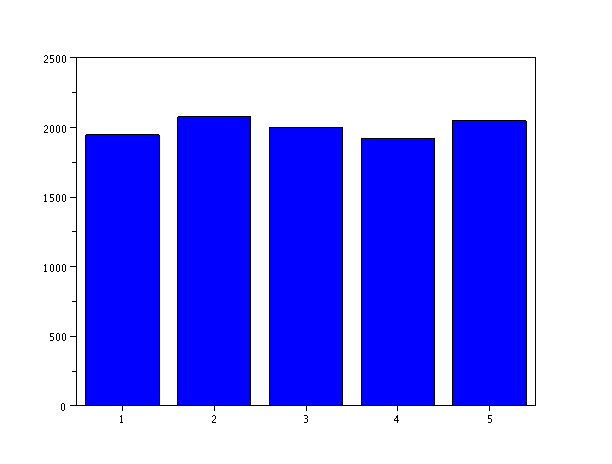
\includegraphics[width=10cm]{introdiscreteprobas/random_0_4.png}
\end{center}
\caption{Distribution of random integers from $0$ to $4$.}
\label{fig-introstats-distributionrandints}
\end{figure}

We emphasize that the previous verifications allow to check that the 
empirical distribution function is the expected one, but that 
does not guarantee that the uniform random number generator 
is of good quality. Indeed, consider the sequence $x_n = n \pmod{5}$. 
This sequence produces uniform integers in the set $\{0,1,\ldots,4\}$, 
but, obviously, is far from being truly random. Testing uniform random 
number generators is a much more complicated problem and will not be 
presented here. 


%%%%%%%%%%%%%%%%%%%%%%%%%%%%%%%%%%%%%%%%%%%%%%%%%%%%%%%%%%%%%%%%%%%%%%%%%%%%%%%%%%%%%%%
\subsection{Simulation of a coin}
\label{introstats-simulatecoin}

Many practical experiments are very difficult to analyze 
by theory and, most of the time, very easy to experiment 
with a computer. In this section, we give an example of a 
coin experiment which is simulated with Scilab. This 
experiment is simple, so that we can check that
our simulation matches the result predicted by theory. 
In practice, when no theory is able to predict a probability,
it is much more difficult to assess the result of simulation.

The following Scilab function generates a random number
with the \scifun{rand} function and use the \scifun{floor}
in order to get a random integer, either 1, associated with "Head",
or 0, associated with "Tail". It prints out the result and returns the 
value.

\lstset{language=scilabscript}
\begin{lstlisting}
// tossacoin --
//   Prints "Head" or "Tail" depending on the simulation.
//   Returns 1 for "Head", 0 for "Tail"
function face = tossacoin ( )
  face = floor ( 2 * rand() );
  if ( face == 1 ) then
    mprintf ( "Head\n" )
  else
    mprintf ( "Tail\n" )
  end
endfunction
\end{lstlisting}

With such a function, it is easy to simulate the toss of a coin.
In the following session, we toss a coin 4 times.
The "seed" argument of the \scifun{rand} is used so that the seed
of the uniform random number generator is initialized to 0. This allows 
to get consistent results across simulations. 

\lstset{language=scilabscript}
\begin{lstlisting}
rand("seed",0)
face = tossacoin ();
face = tossacoin ();
face = tossacoin ();
face = tossacoin ();
\end{lstlisting}

The previous script produces the following output.

\lstset{language=scilabscript}
\begin{lstlisting}
Tail
Head
Tail
Tail
\end{lstlisting}

Assume that we are tossing a fair coin 10 times.
What is the probability that we get exactly 5 heads ?

This is a Bernoulli process, where the number of trials is 
$n=10$ and the probability is $p=5$. The probability of getting
exactly $j=5$ heads is given by the binomial distribution and is 
\begin{eqnarray}
P(\textrm{"exactly 5 heads in 10 toss"})&=&b(10,1/2,5) \\
&=& \choosefun{10}{5} p^5 q^{10-5},
\end{eqnarray}
where $p=1/2$ and $q=1-p$.
The expected probability is therefore 
\begin{eqnarray}
P(\textrm{"exactly 5 heads in 10 toss"})&\approx & 0.2460938.
\end{eqnarray}

The following Scilab session shows how to perform the simulation.
Then, we perform 
10000 simulations of the process. The \scifun{floor} function is used 
in combination with the \scifun{rand} function to generate integers in the 
set $\{0,1\}$. The \scifun{sum} allows to count the number of 
heads in the experiment. If the number of heads is equal to 5, 
the number of successes is updated accordingly.

\lstset{language=scilabscript}
\begin{lstlisting}
-->rand("seed",0);
-->nb = 10000;
-->success = 0;
-->for i = 1:nb
-->  faces = floor ( 2 * rand(1,10) );
-->  nbheads = sum(faces);
-->  if ( nbheads == 5 ) then
-->    success = success + 1;
-->  end
-->end
-->pc = success / nb
 pc  =
    0.2507
\end{lstlisting}

The computed probability is $P=0.2507$ while the theory 
predicts $P=0.2460938$, which means that there is lest than 
two significant digits.
It can be proved that when we simulate an experiment of this type $n$ times, 
we can expect that the error is less or equal to $\frac{1}{\sqrt{n}}$ at least $95\%$ of the time.
With $n=10000$ simulations, this error corresponds to $0.01$, which is the 
accuracy of our experiment.

%%%%%%%%%%%%%%%%%%%%%%%%%%%%%%%%%%%%%%%%%%%%%%%%%%%%%%%%%%%%%%%%%%%%%%%%%%%%%%%%%%%%
\section{Acknowledgments}

I would like to thank John Burkardt for his comments about the numerical 
computation of the permutation function.



%%%%%%%%%%%%%%%%%%%%%%%%%%%%%%%%%%%%%%%%%%%%%%%%%%%%%%%%%%%%%%%%%%%%%%%%%%%%%%%%%%%%%%%

\section{References and notes}

The material for section \ref{introstats-setsrandomvars} is 
presented in \cite{Loeve1963}, chapter 1, "Set, spaces and measures".
The same presentation is given in \cite{introprobasGrinsteadSnell}, section
1.2, "Discrete probability distributions". The example \ref{introstats-die6faces}
is given in \cite{introprobasGrinsteadSnell}.

The equations \ref{introstats-pzerone}, \ref{introstats-pomegaone} and 
\ref{introstats-pdisjointssum} are at the basis of the probability 
theory so that in \cite{Ross1987}, these properties are stated as axioms.

In some statistics books, such as \cite{montecarlomethodsHammersleyHandscomb}
for example, the union of the sets $A$ and $B$ is denoted by the sum $A+B$, and 
the intersection of sets is denoted by the product $AB$.
We did not use these notations in this document.

Combinatorics topics presented in section \ref{introstats-chap-combinatorics} 
can be found in \cite{introprobasGrinsteadSnell}, chapter 3, "Combinatorics".
The example of Poker hands is presented in \cite{introprobasGrinsteadSnell},
while the probabilities of all Poker hands can be found in 
Wikipedia \cite{wiki:pokerprobas}.

The gamma function presented in section \ref{section-gammafun} is covered
in many textbook, as in \cite{AbramowitzStegun1972}. An in-depth presentation of 
the gamma function is done in \cite{SebahGourdon2002}.

Some of the section \ref{introstats-simulation} which introduces
to random number generators is based on \cite{artcomputerKnuthVol2}.





%%%%%%%%%%%%%%%%%%%%%%%%%%%%%%%%%%%%%%%%%%%%%%%%%%%%%%%%%%%%%%%%%%%%%%%%%%%%%%%%%%%%




%% Bibliography

\addcontentsline{toc}{section}{Bibliography}
\bibliographystyle{plain}
\bibliography{introdiscreteprobas}

\addcontentsline{toc}{section}{Index}
\printindex

\end{document}

